\newpage
%
\subsection{Списание материалов}
\label{bp:MatOutput}

\subsubsection{Списание бумаги и картона}

 На основании печатного варианта задания на гофроагрегат Бригадир формирует для водителя погрузчика задание на подачу сырья к раскатам (рис. \ref{pic:V план для карщика}). При этом Бригадир учитывает сообщения отдела планирования производства о разрешенных заменах сырья (рис. \ref{pic:V задание с ЦУ от плановика}) для каждого задания и общий список возможных замен (рис. \ref{pic:V примечания по заменам сырья}). Бригадир имеет возможность в системе 1С: УПП сформировать отчет по остаткам сырья на складе (рис. \ref{pic:V оценка наличия сырья}).

Водитель погрузчика при подаче рулонов со склада производит сканирование штрихкода на бирке рулона. На ТСД формируется документ перемещения, таким образом фиксируется факт подачи сырья на производство. На момент аудита внутризаводские бирки не используются, внутризаводские номера рулонов не применяются.

Машинист гофроагрегата устанавливает рулон на соответствующий раскат, срезает бирку и оставляет ее на пульте управления (рис. \ref{pic:V раскаты}). При сканировании штрихкода на бирке рулона (рис. \ref{pic:V Сканер на ГА}) в системе 1С: УПП фиксируется информация о установке рулона на определенный раскат.

На гофроагрегате  реализована систем по учету количества погонных метров, затраченных с каждого рулона (рис. \ref{pic:V Метраж рулонов}). При снятии рулона машинист в системе 1С: УПП фиксирует расход сырья (рис. \ref{pic:V фиксация на раскатах}). Если рулон использован не полностью, то машинист наклеивает обратно бирку и водитель погрузчика отвозит рулон на место хранения около гофроагрегата (рис. \ref{pic:V недомоты}). На склад рулоны не вывозятся. Если рулон выработан полностью, то машинист оставляет бирку для учетчика у пульта раската. 
 Ежедневно учетчик забирает бирки и в системе 1С: УПП проверяет правильность занесения информации по рулонам и при необходимости производит анализ и корректировку (рис. \ref{pic:IV.2.}).   
Списание сырья на конкретный заказ не производится. Списание порулонно в системе 1С: УПП производится бухгалтерией ежедневно. 

%Машинист гофроагрегата создает потребность в сырье (рис. \ref{pic:d38}), которую передает с водителем на склад материалов.
%Кладовщик перемещает материалы на основании потребности, списывает остатки в системе СБИС.

%Кладовщик пишет отчет по остаткам в таблице MS Excel (рис. \ref{pic:d38_1}). 
%Остатки в системе СБИС ведутся, но кладовщик не проверяет остатки в системе. Отчет формируется более 5 минут.
%По таблице \ref{pic:d38_1} кладовщик определяет остатки по сырью и передает инрис.цию машинисту гофроагрегата.
%Кладовщик в конце смены списывает рулоны бумаги и картона в форме MS Excel (рис. \ref{pic:d38_1}).
%По форме \ref{pic:d38} кладовщик записывает номера рулонов, которые были списаны в производство (рис. \ref{pic:d39}).
%В течение смены кладовщик списывает в системе СБИС рулоны в документ  “Накладная перемещения”.
%В системе СБИС кладовщик списывает рулон в метрах квадратных.

%Остатки по рулонам обратно на склад не перемещаются и остаются в производстве.

%По факту использования рулонов на гофроагрегате операторы на раскатах отмечают использованные рулоны в отчете по каждому раскату (рис. \ref{pic:d9}).
%В конце смены отчет с каждого раската мастер передает в БППП.
%Инженер-экономист в БППП на основании формы \ref{pic:d9} выполняет списание сырья в производство в системе СБИС.
%Инженер-экономист в БППП на основании формы \ref{pic:d9} создает отчет по браку (рис. \ref{pic:d10}) и передает в отдел ОТК.
%Брак считается по среднему.

%Инженер-экономист в БППП списывает рулоны в (рис. \ref{pic:d12}) в системе СБИС. 
%Инженер-экономист в БППП создает отчет по учету сырья (рис. \ref{pic:d13}) директору и начальнику производства.

\subsection{Учет вспомогательных материалов}

Учет вспомогательных материалов ведется в системе 1С: УПП. Контроль и предоставление данных в бухгалтерию осуществляет технологический отдел. Списание производится ''котловым'' методом один раз в месяц на  основании информации из бумажных отчетов от производства (рис. \ref{pic:V учет расхода крахмала}).


%Каждый день техник по учету БППП определяет инрис.цию по остаткам вспомогательных материалов на складе.
%Расходы по крахмалу и прочим вспомогательным материалам техник по учету БППП списывает в системе СБИС заносит из форм \ref{pic:d18}, \ref{pic:d17_1}.
%В конце каждого месяца техник по учету в системе СБИС формирует отчет по обороту материалов (рис. \ref{pic:d19}) и передает в бухгалтерию Предприятия.

\textbf{Списание краски}

Расход готовой краски на предприятии составляет 2-2,5 тонны в месяц. ПРЕДПРИЯТИЕ закупает пигменты для приготовления краски с использованием станции смешения. Контроль и предоставление данных в бухгалтерию осуществляет технологический отдел. Списание производиться в системе 1С: УПП ''котловым'' методом  один раз в месяц на  основании информации из бумажных отчетов от производства.

%Для себя техники ведут учет краски в программе по отчету (рис. \ref{pic:a7}) в системе СБИС. Раз в месяц для списания техники передают отчеты по использованию краски в бухгалтерию предприятия (рис. \ref{pic:a7}, \ref{pic:a9}). Списывает краску бухгалтерия в программе СБИС. 


% После использования краски машинисты взвешивают ведра с  остатками на весах (рис. \ref{pic:a14}) и на ведро машинист клеит ярлык с весом (рис. \ref{pic:a13}). Краска на каждой линии хранится на своем месте. Разбавленная краска не учитывается и остается в рабочих ведрах. 


% После взвешивания краски машинист пишет в документе ''Сменный рапорт машиниста'' количество использованной краски (рис. \ref{pic:a68}). На основании этих данных мастер смены ежедневно вносит данные для списания краски в системе 1С:УНФ.


% Краску списывает мастер в системе 1С:УНФ ежедневно на основании документа ''Сменный рапорт машиниста'', в который машинист вписывает руками количество израсходованной краски.  


% Списание вспомогательных материалов (клей, стрейч, скобы, ленты) выполняет мастер в конце месяца на основании данных инвентаризации и передает данные в бухгалтерию. Бухгалтер списывает  вспомогательных материалов в системе 1С:УНФ документом ''Списание ТМЦ''.
% % Хранение клея (11).

% Списание поддонов определяется по количеству переданных на склад. Учет поддонов выполняет мастер. Размеры поддонов определяются из упаковки.

% Раз в месяц мастер выполняет списание материалов (заготовки) и списание недопоставки от поставщика заготовки и списание на образцы (рис. \ref{pic:a74}, \ref{pic:a75}, \ref{pic:a76}). Все списания мастер сверяет с кладовщиком склада.

% \subsubsection{Списание бумаги и картона}

\newpage
\begin{figure}
\begin{center}
 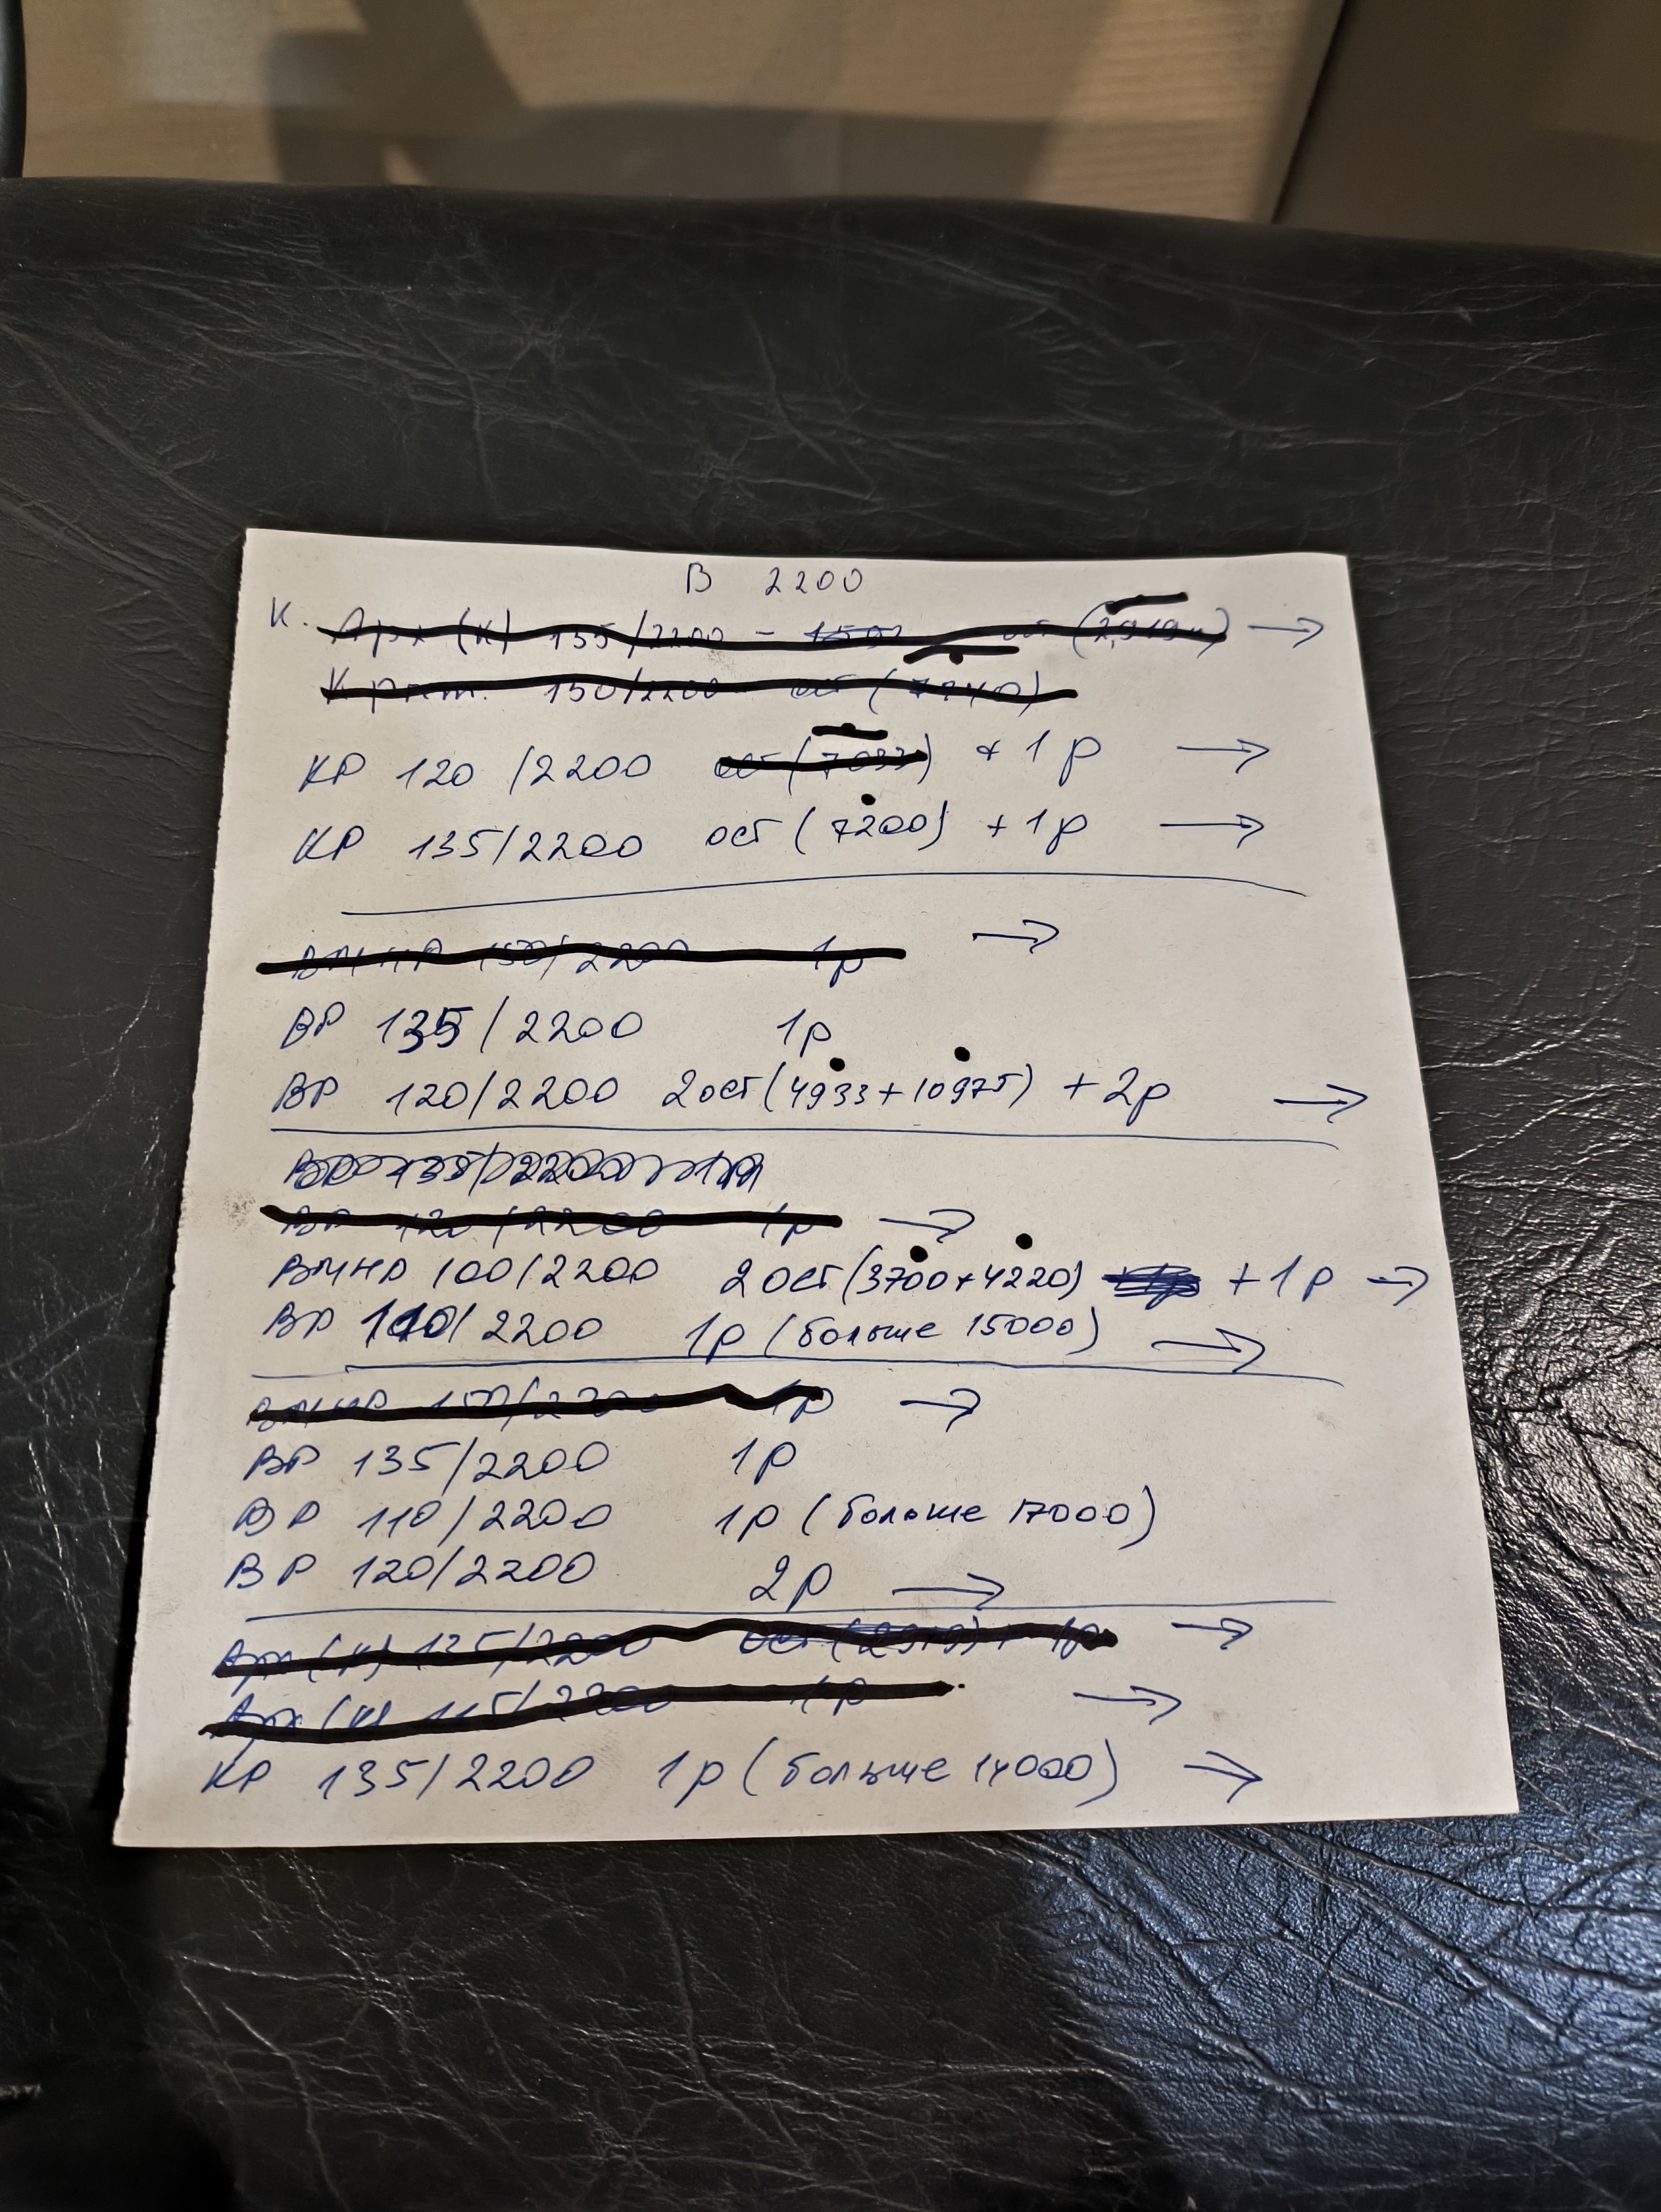
\includegraphics[height=0.9\textheight, keepaspectratio]{Pics/V план для карщика.jpg}
\end{center}
 \caption{План подачи сырья}
 \label{pic:V план для карщика}
\end{figure}

\newpage
\begin{figure}
\begin{center}
 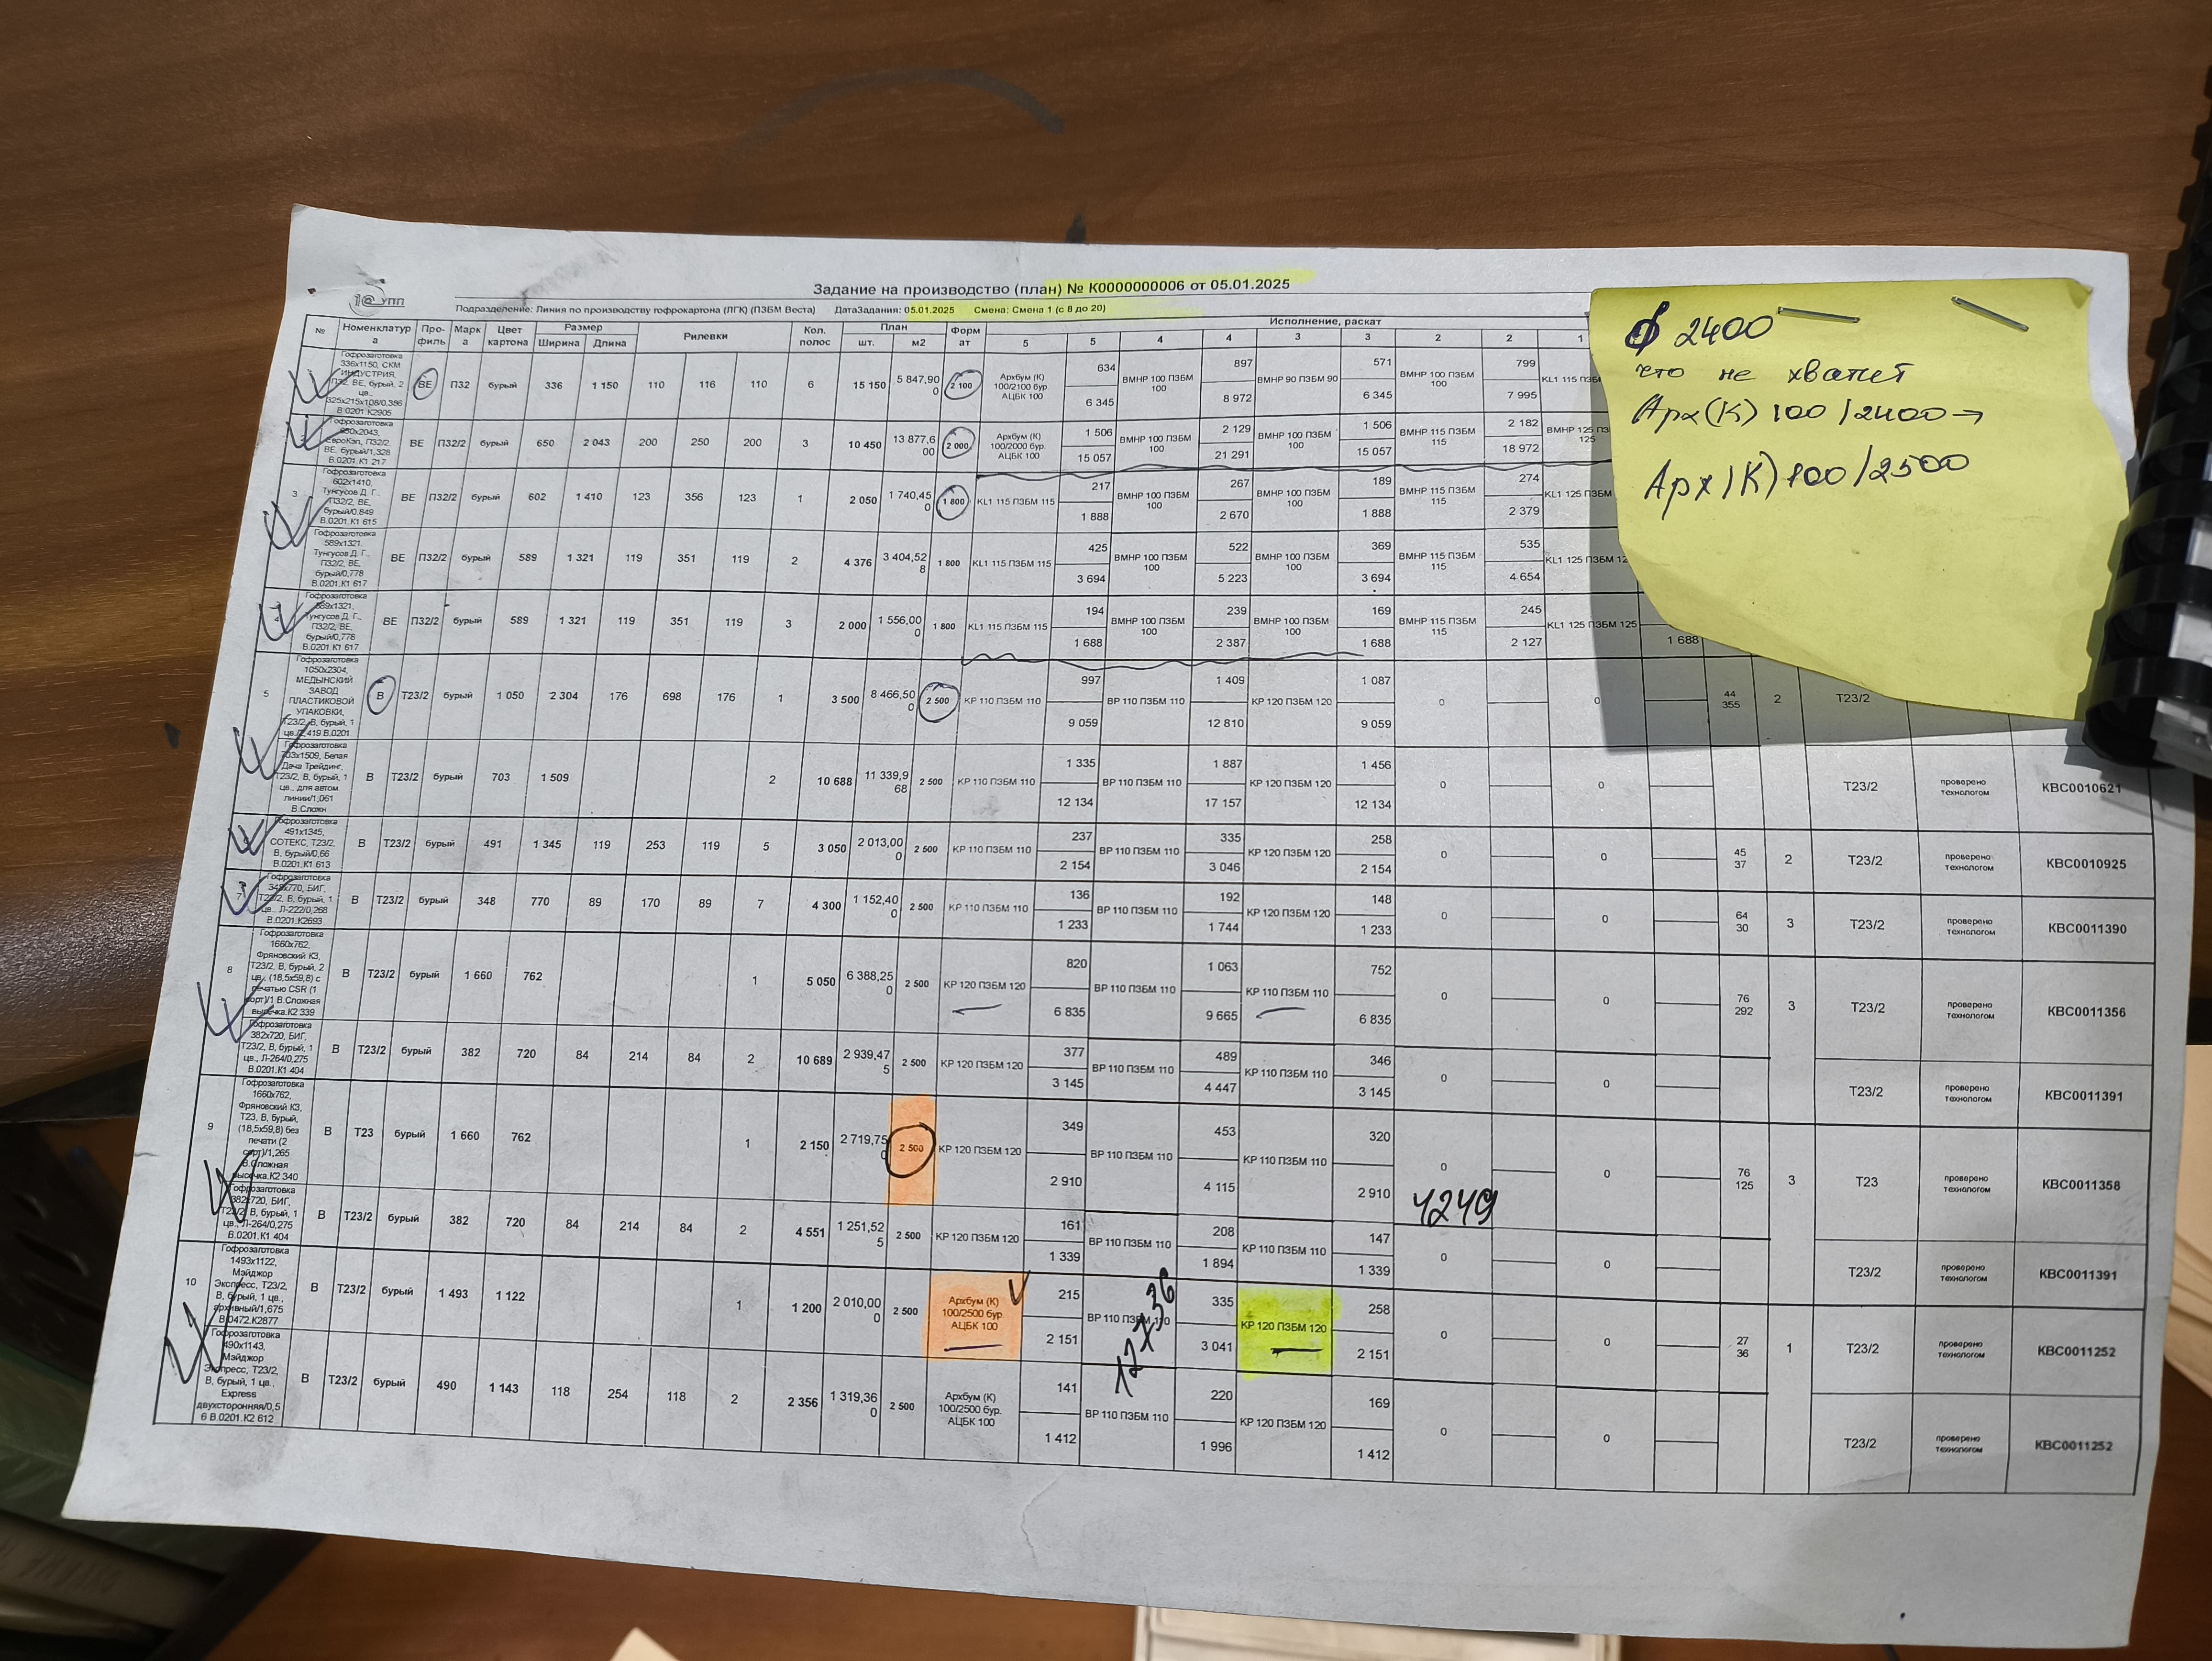
\includegraphics[height=0.4\textheight, keepaspectratio]
 {Pics/V задание с ЦУ от плановика.jpg }
\end{center}
 \caption{Задание на ГА}
 \label{pic:V задание с ЦУ от плановика}
\end{figure}

\newpage
\begin{figure}
\begin{center}
 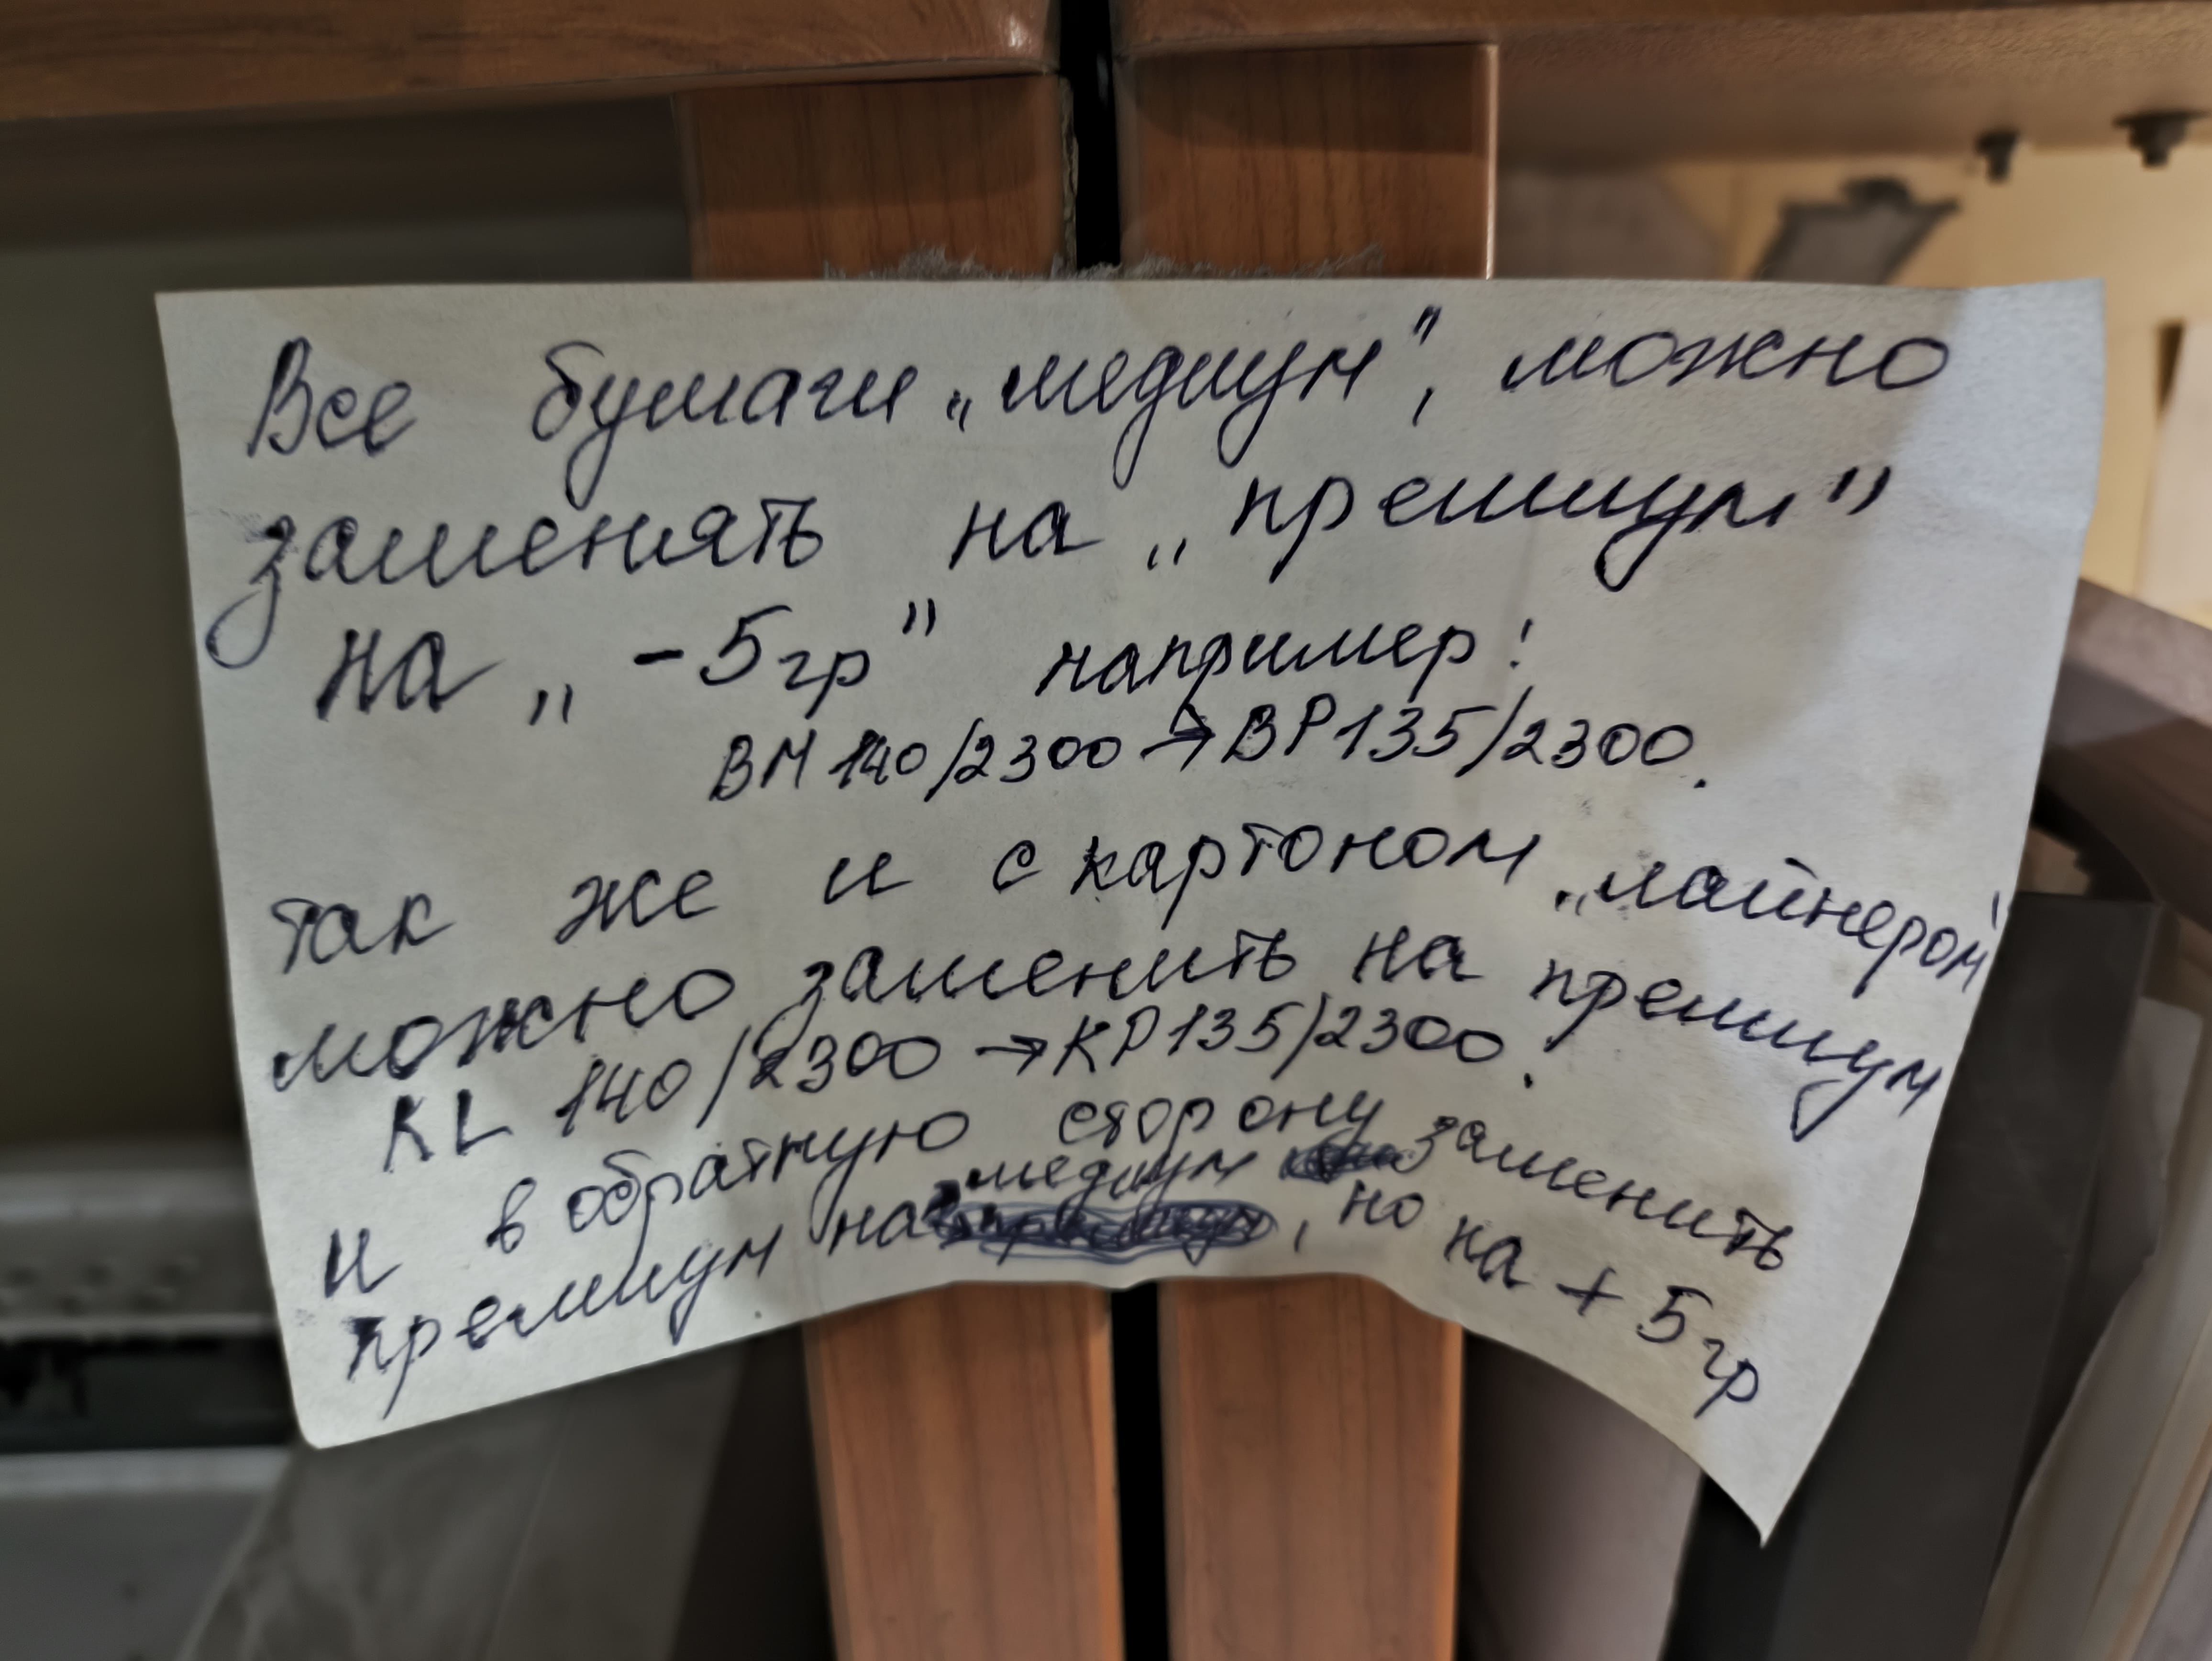
\includegraphics[height=0.4\textheight, keepaspectratio]{Pics/V примечания по заменам сырья.jpg}
\end{center}
 \caption{Список возможных замен}
 \label{pic:V примечания по заменам сырья}
\end{figure}
%
\begin{figure}
\begin{center}
 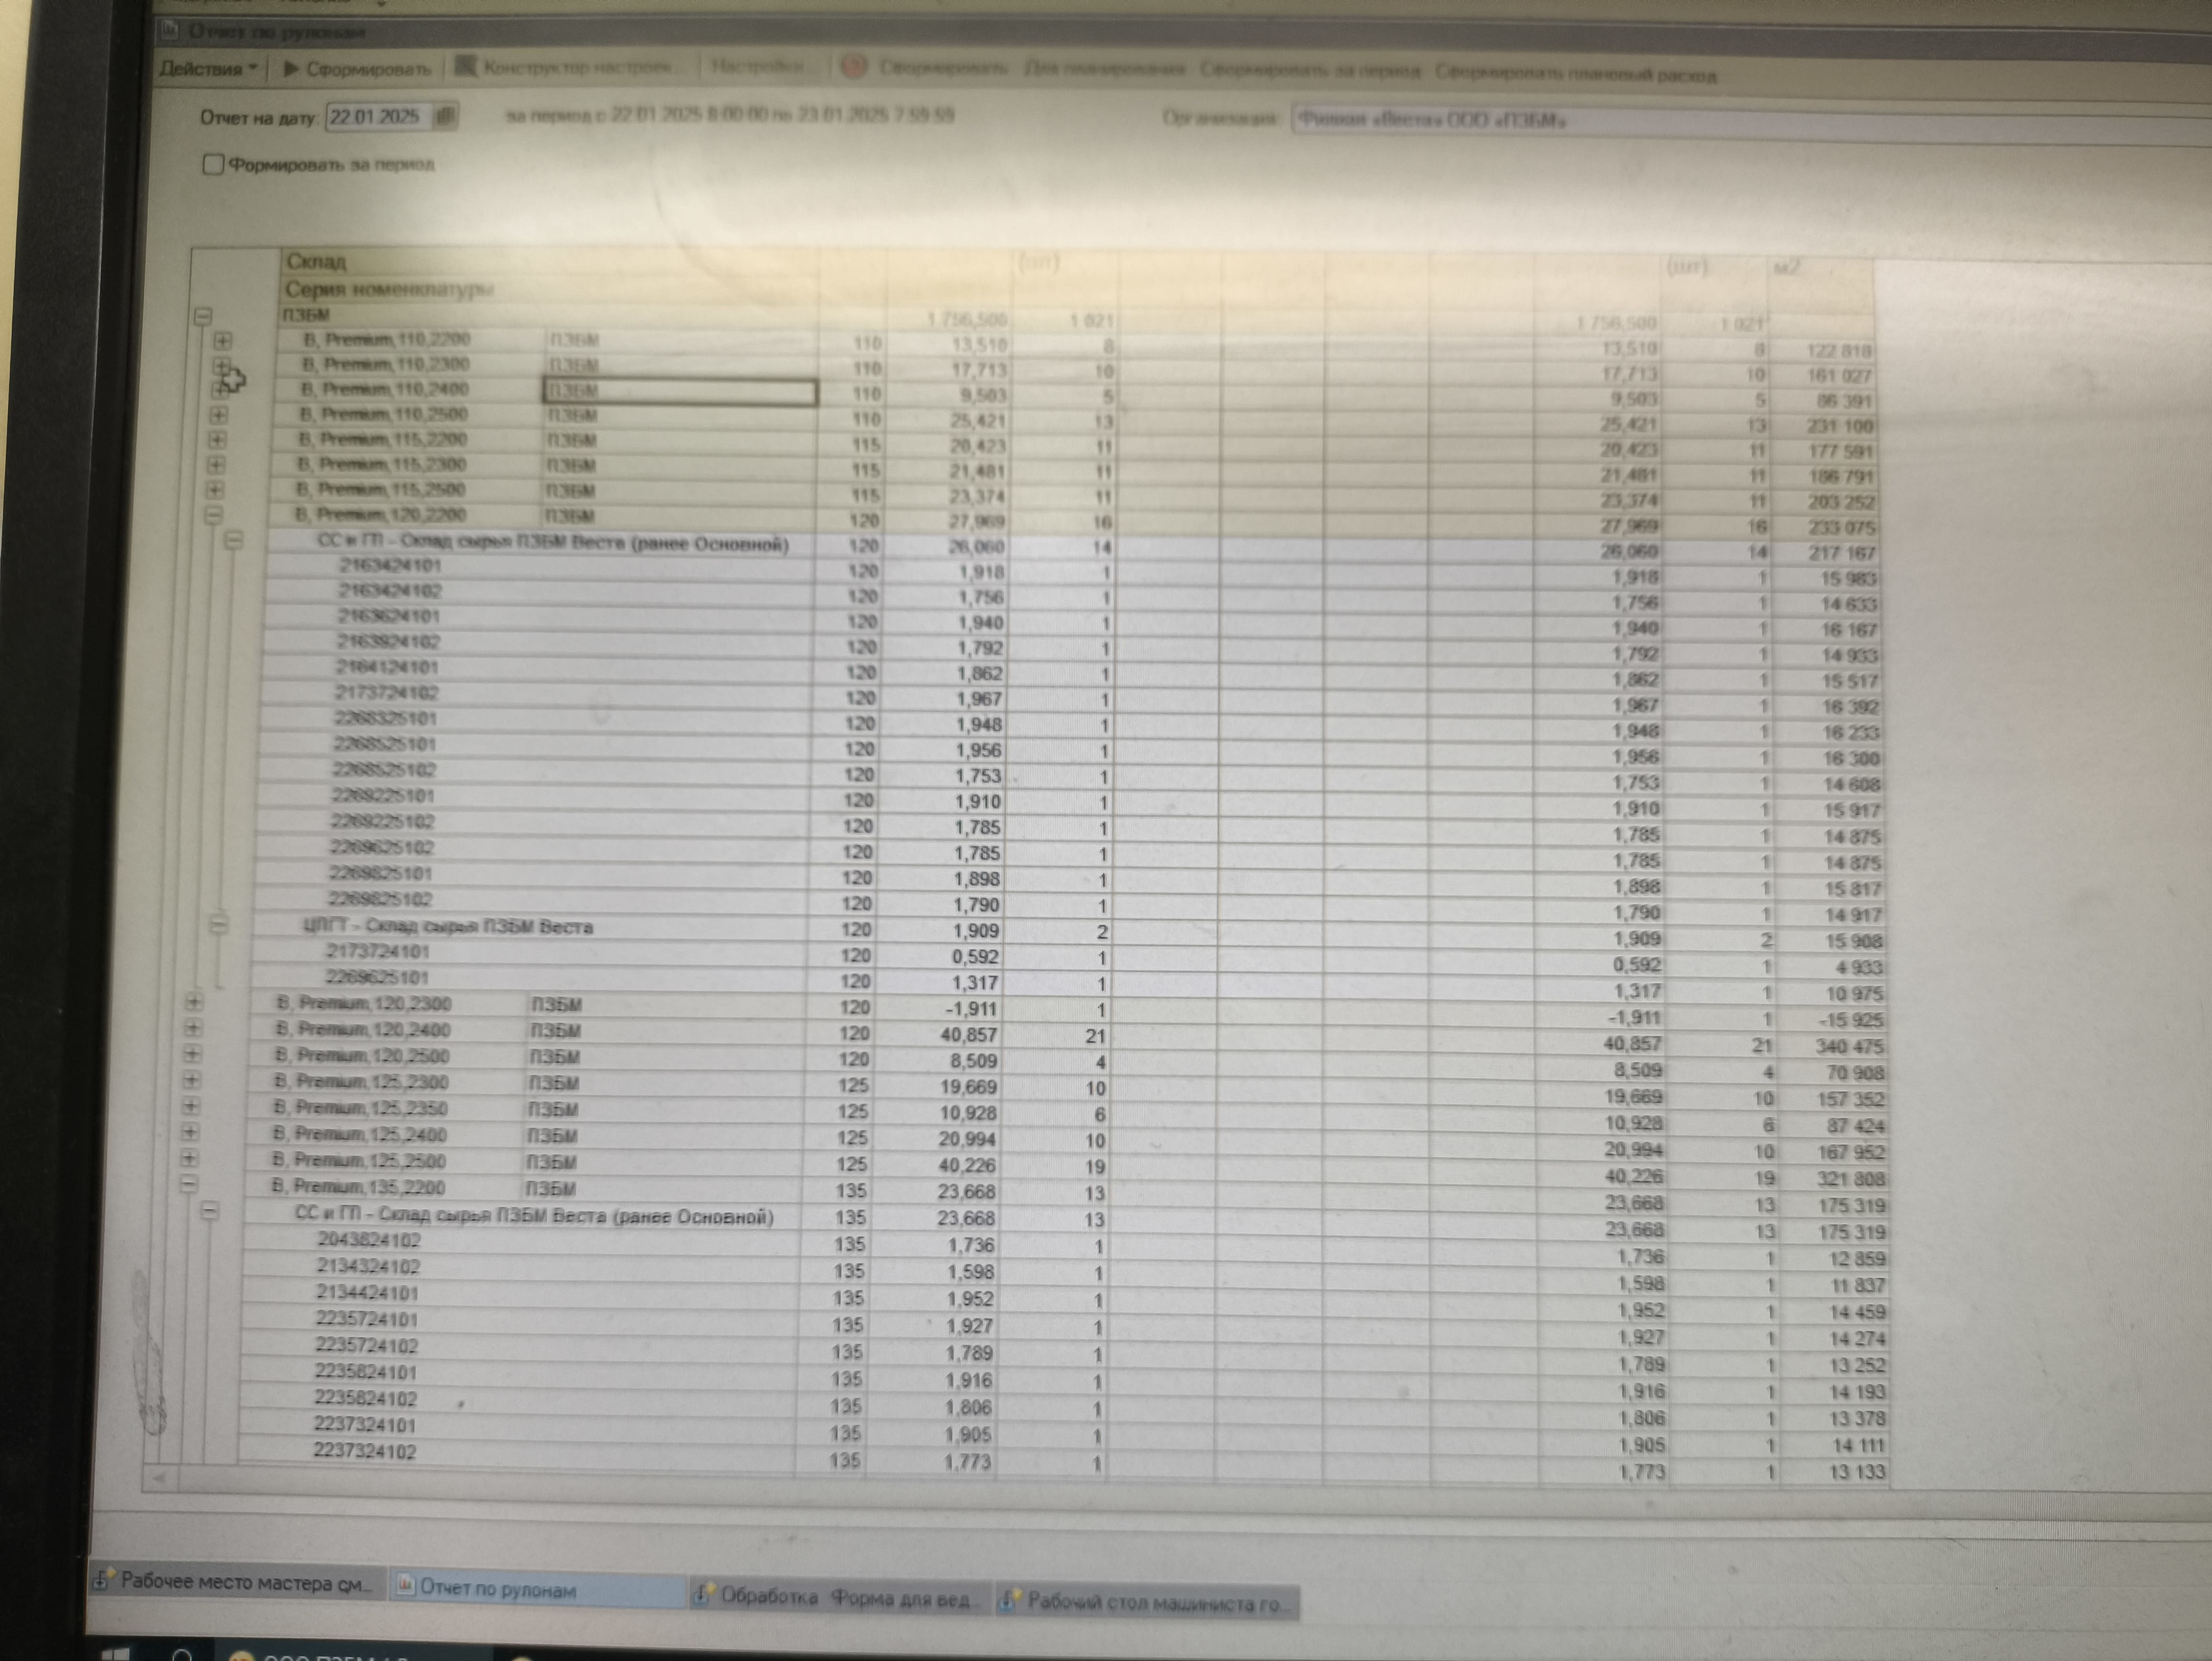
\includegraphics[height=0.4\textheight, keepaspectratio]{Pics/V оценка наличия сырья.jpg}
\end{center}
 \caption{Отчет по рулонам в системе 1С: УПП}
 \label{pic:V оценка наличия сырья}
\end{figure}

\begin{figure}
\begin{center}
 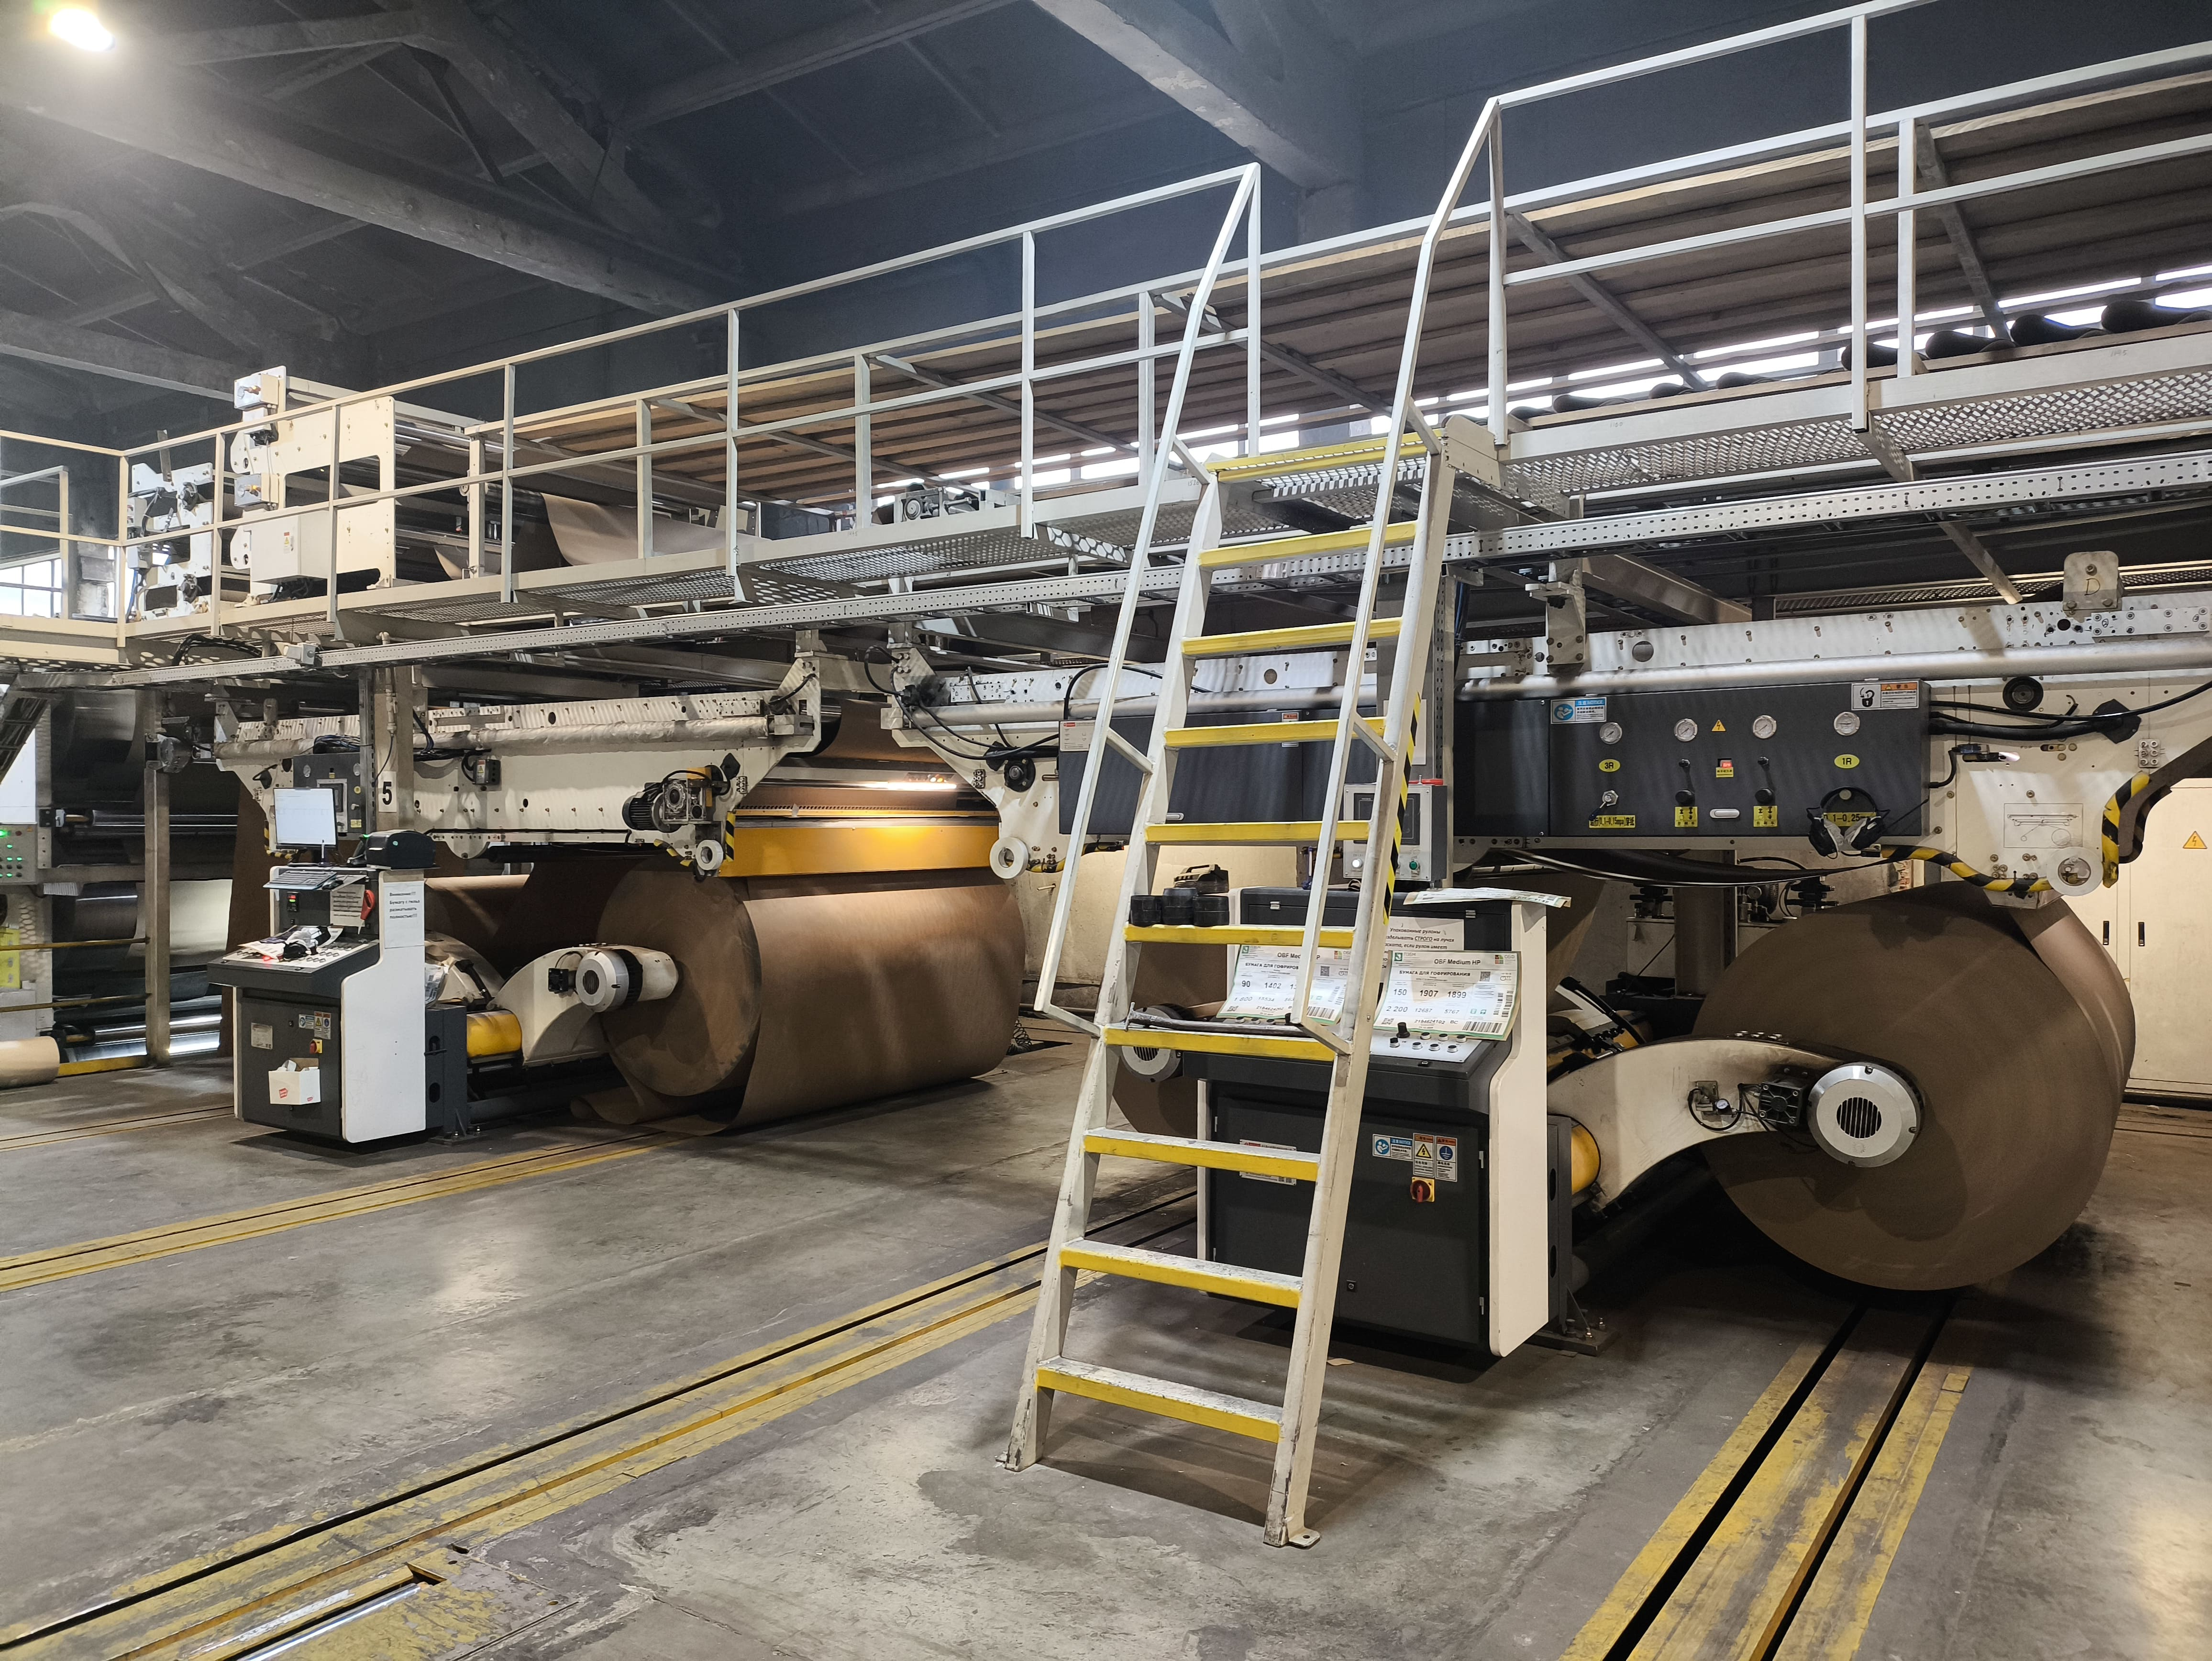
\includegraphics[height=0.4\textheight, keepaspectratio]{Pics/V раскаты.jpg}
\end{center}
 \caption{Хранение бирок на рулоны на гофроагрегате}
 \label{pic:V раскаты}
\end{figure}

\begin{figure}
\begin{center}
 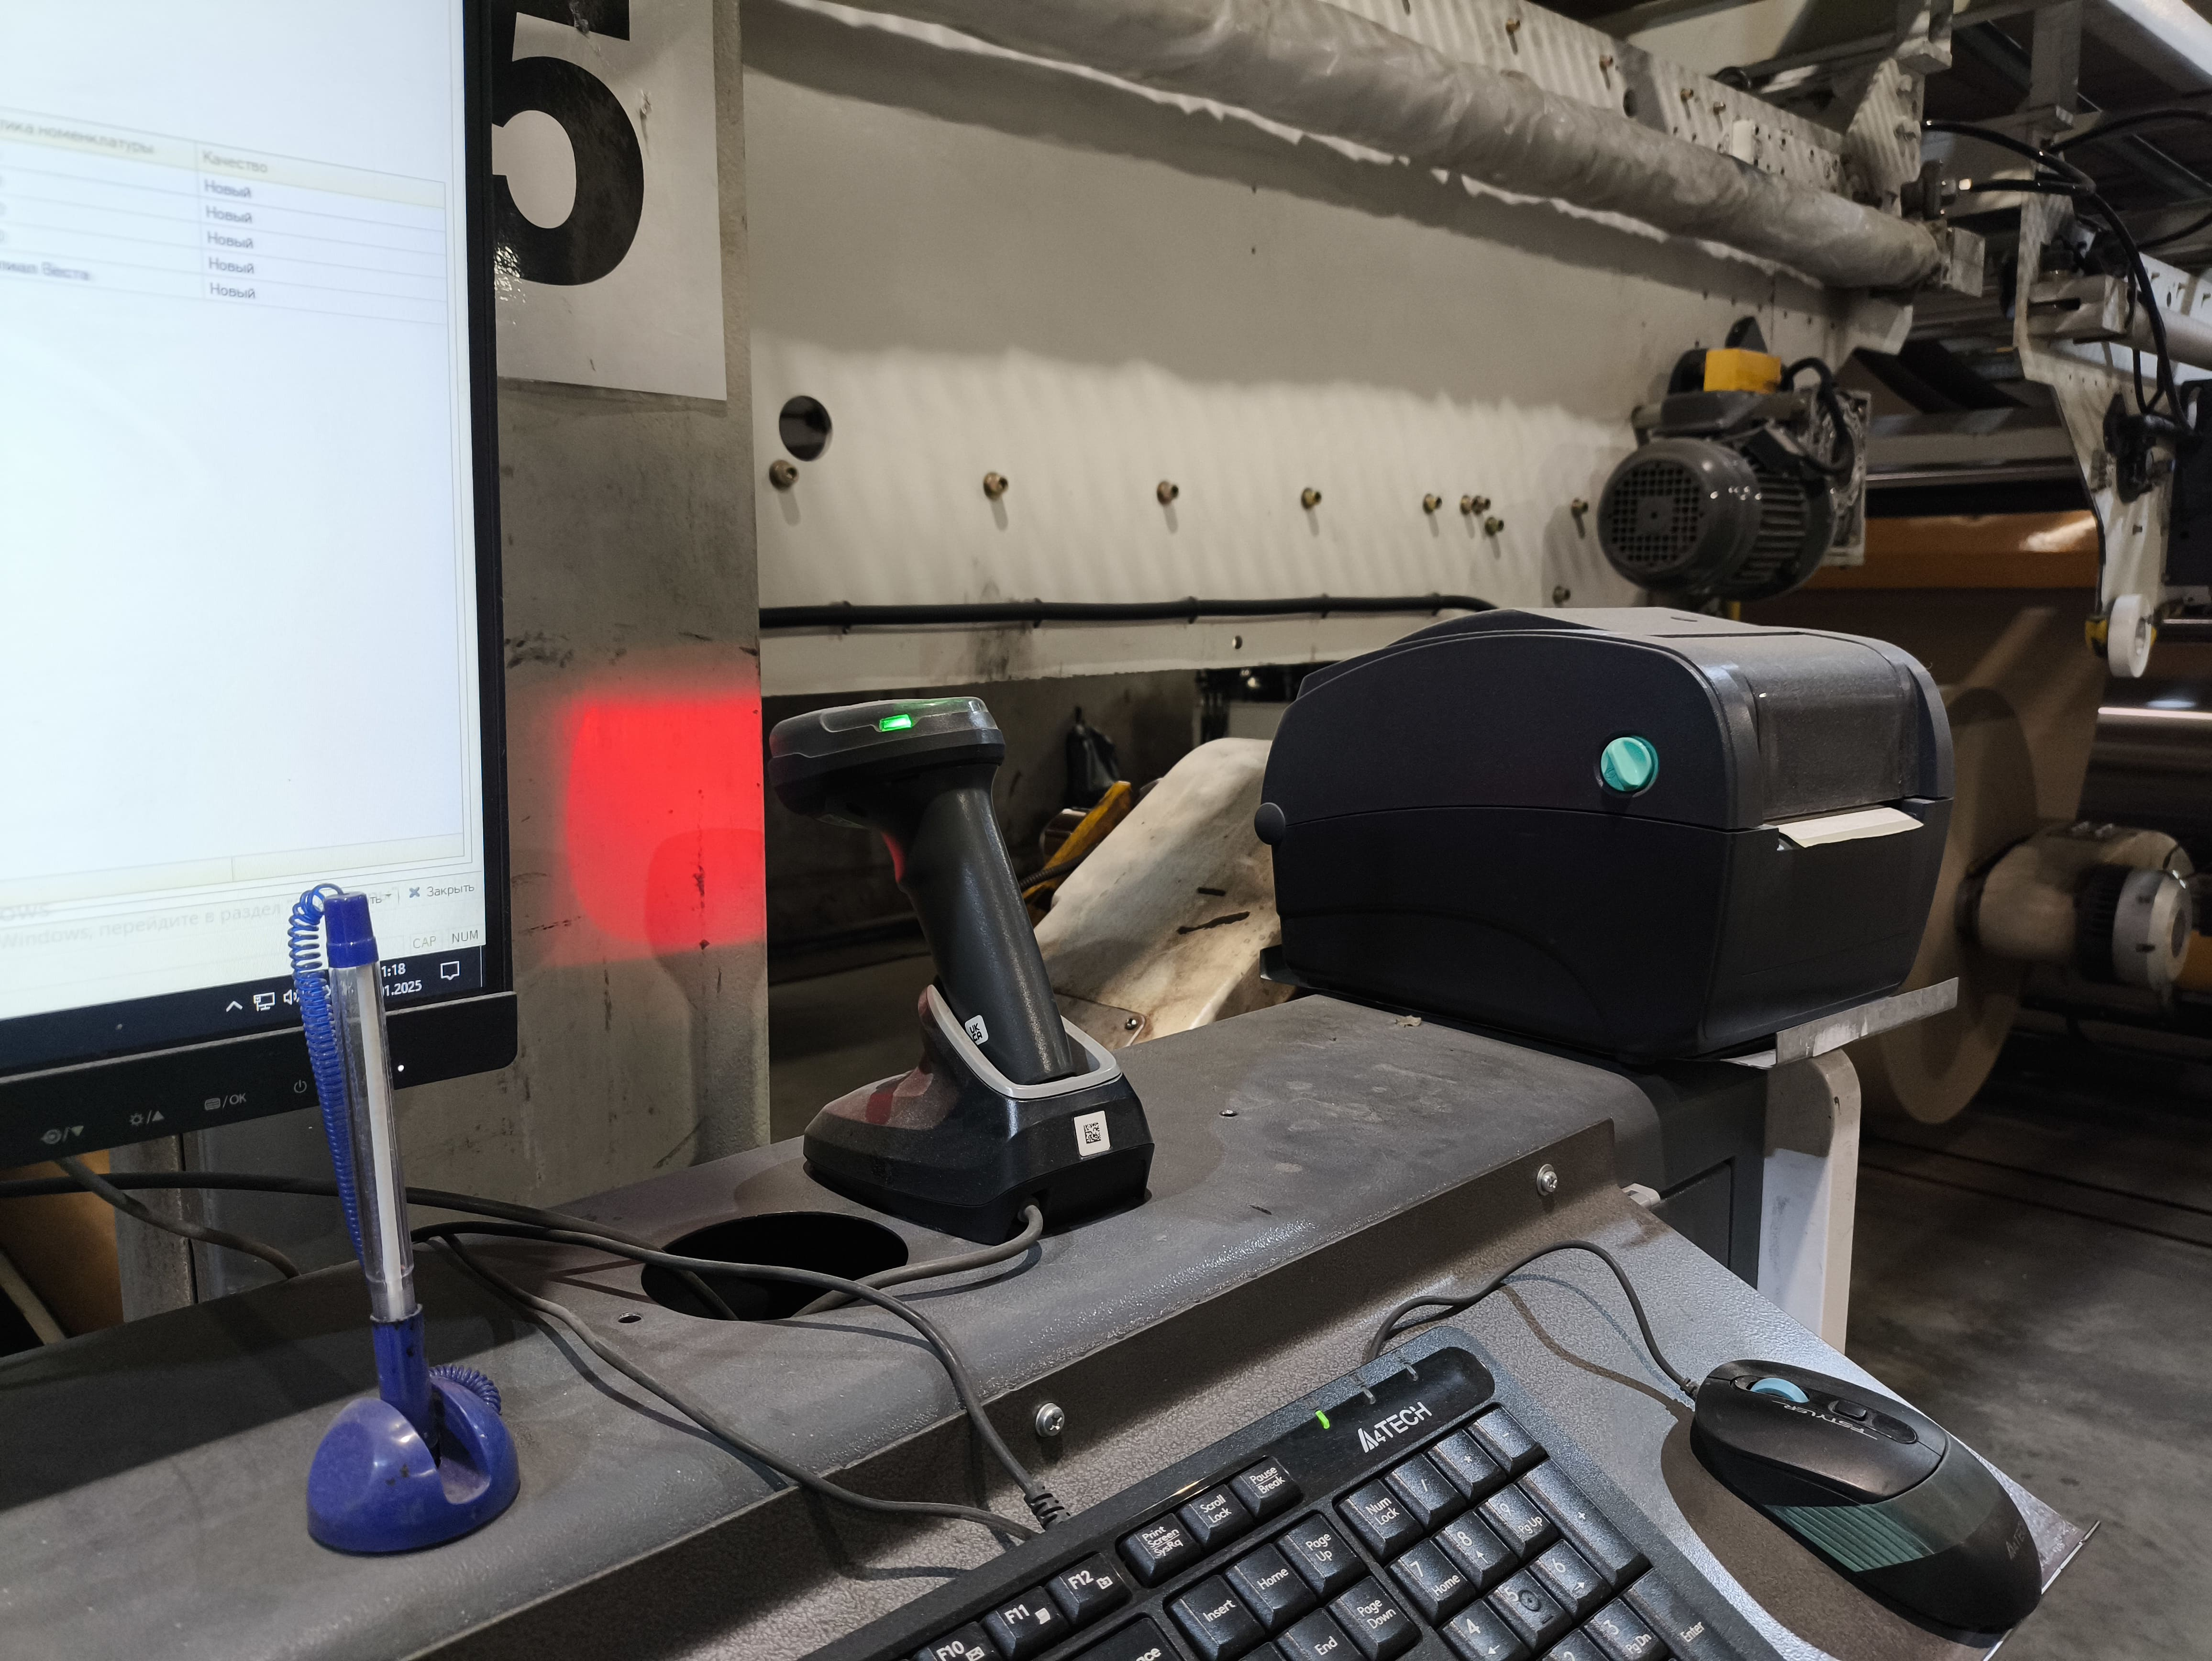
\includegraphics[height=0.4\textheight, keepaspectratio]{Pics/V Сканер на ГА.jpg}
\end{center}
 \caption{Сканер на пульте раската}
 \label{pic:V Сканер на ГА}
\end{figure}

\begin{figure}
\begin{center}
 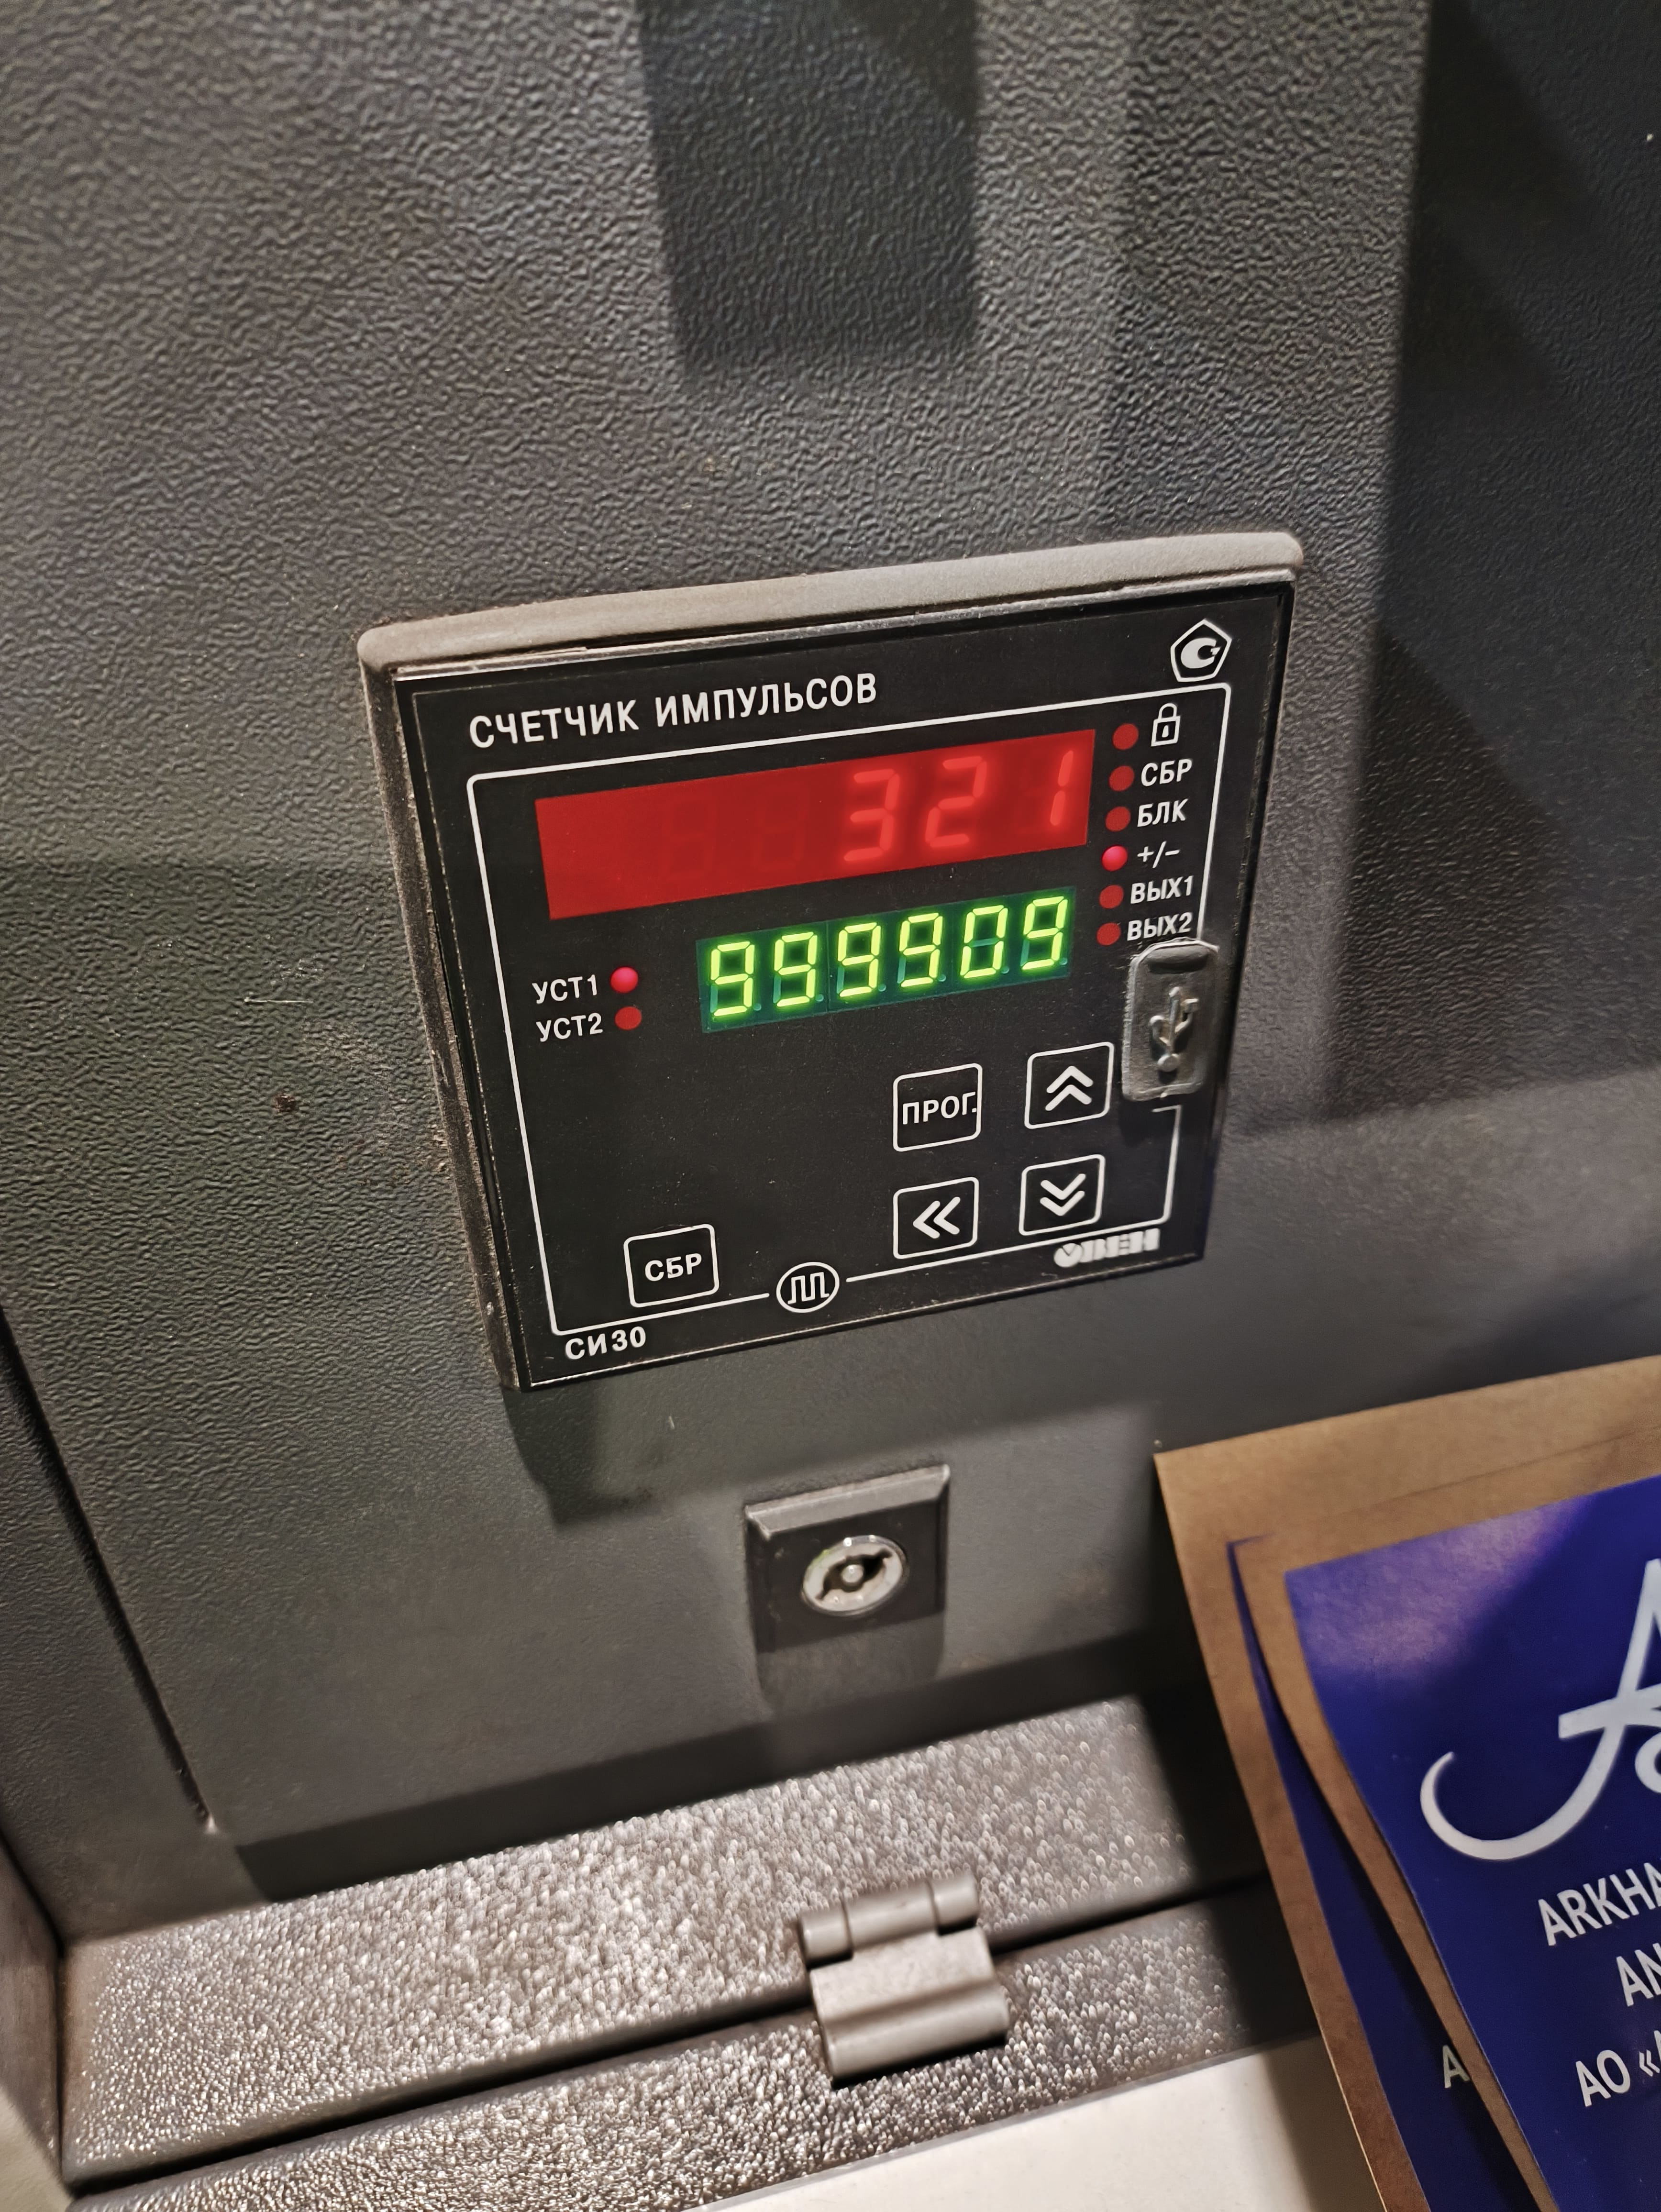
\includegraphics[height=0.4\textheight, keepaspectratio]{Pics/V Метраж рулонов.jpg}
\end{center}
 \caption{Счетчик погонных метров}
 \label{pic:V Метраж рулонов}
\end{figure}

\begin{figure}
\begin{center}
 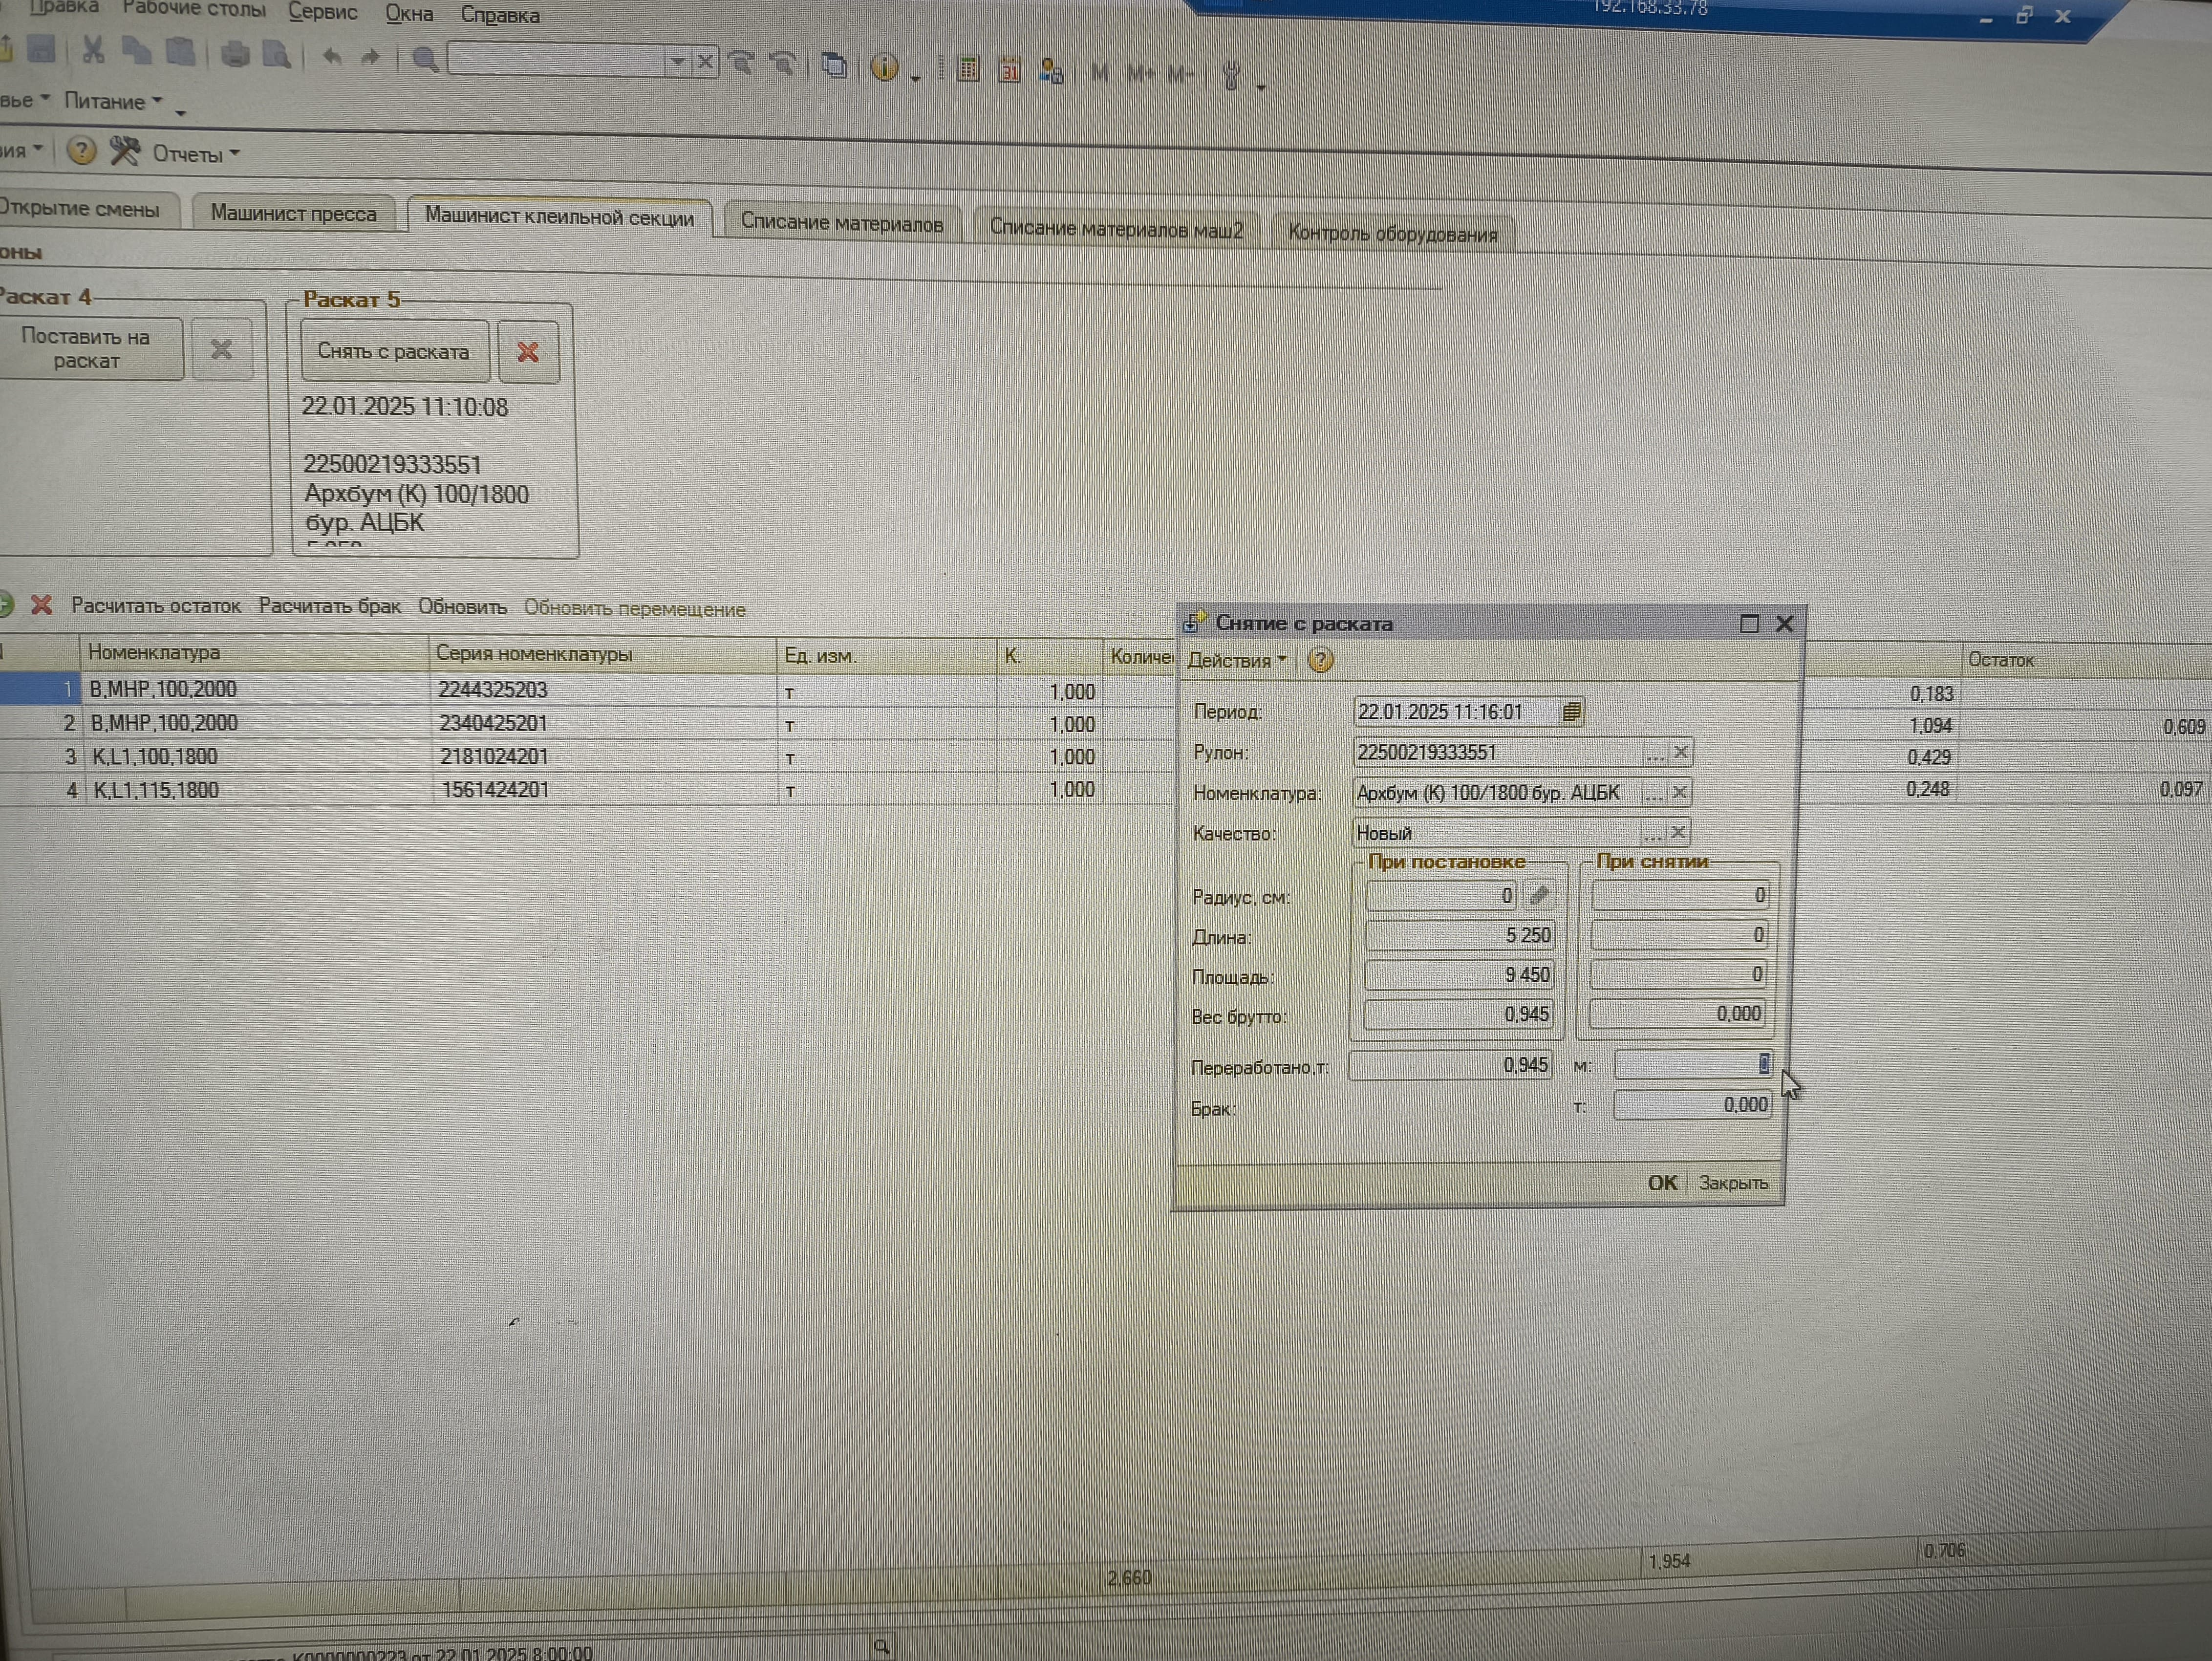
\includegraphics[height=0.4\textheight, keepaspectratio]{Pics/V фиксация на раскатах.jpg}
\end{center}
 \caption{Фиксация расхода сырья}
 \label{pic:V фиксация на раскатах}
\end{figure}

\begin{figure}
\begin{center}
 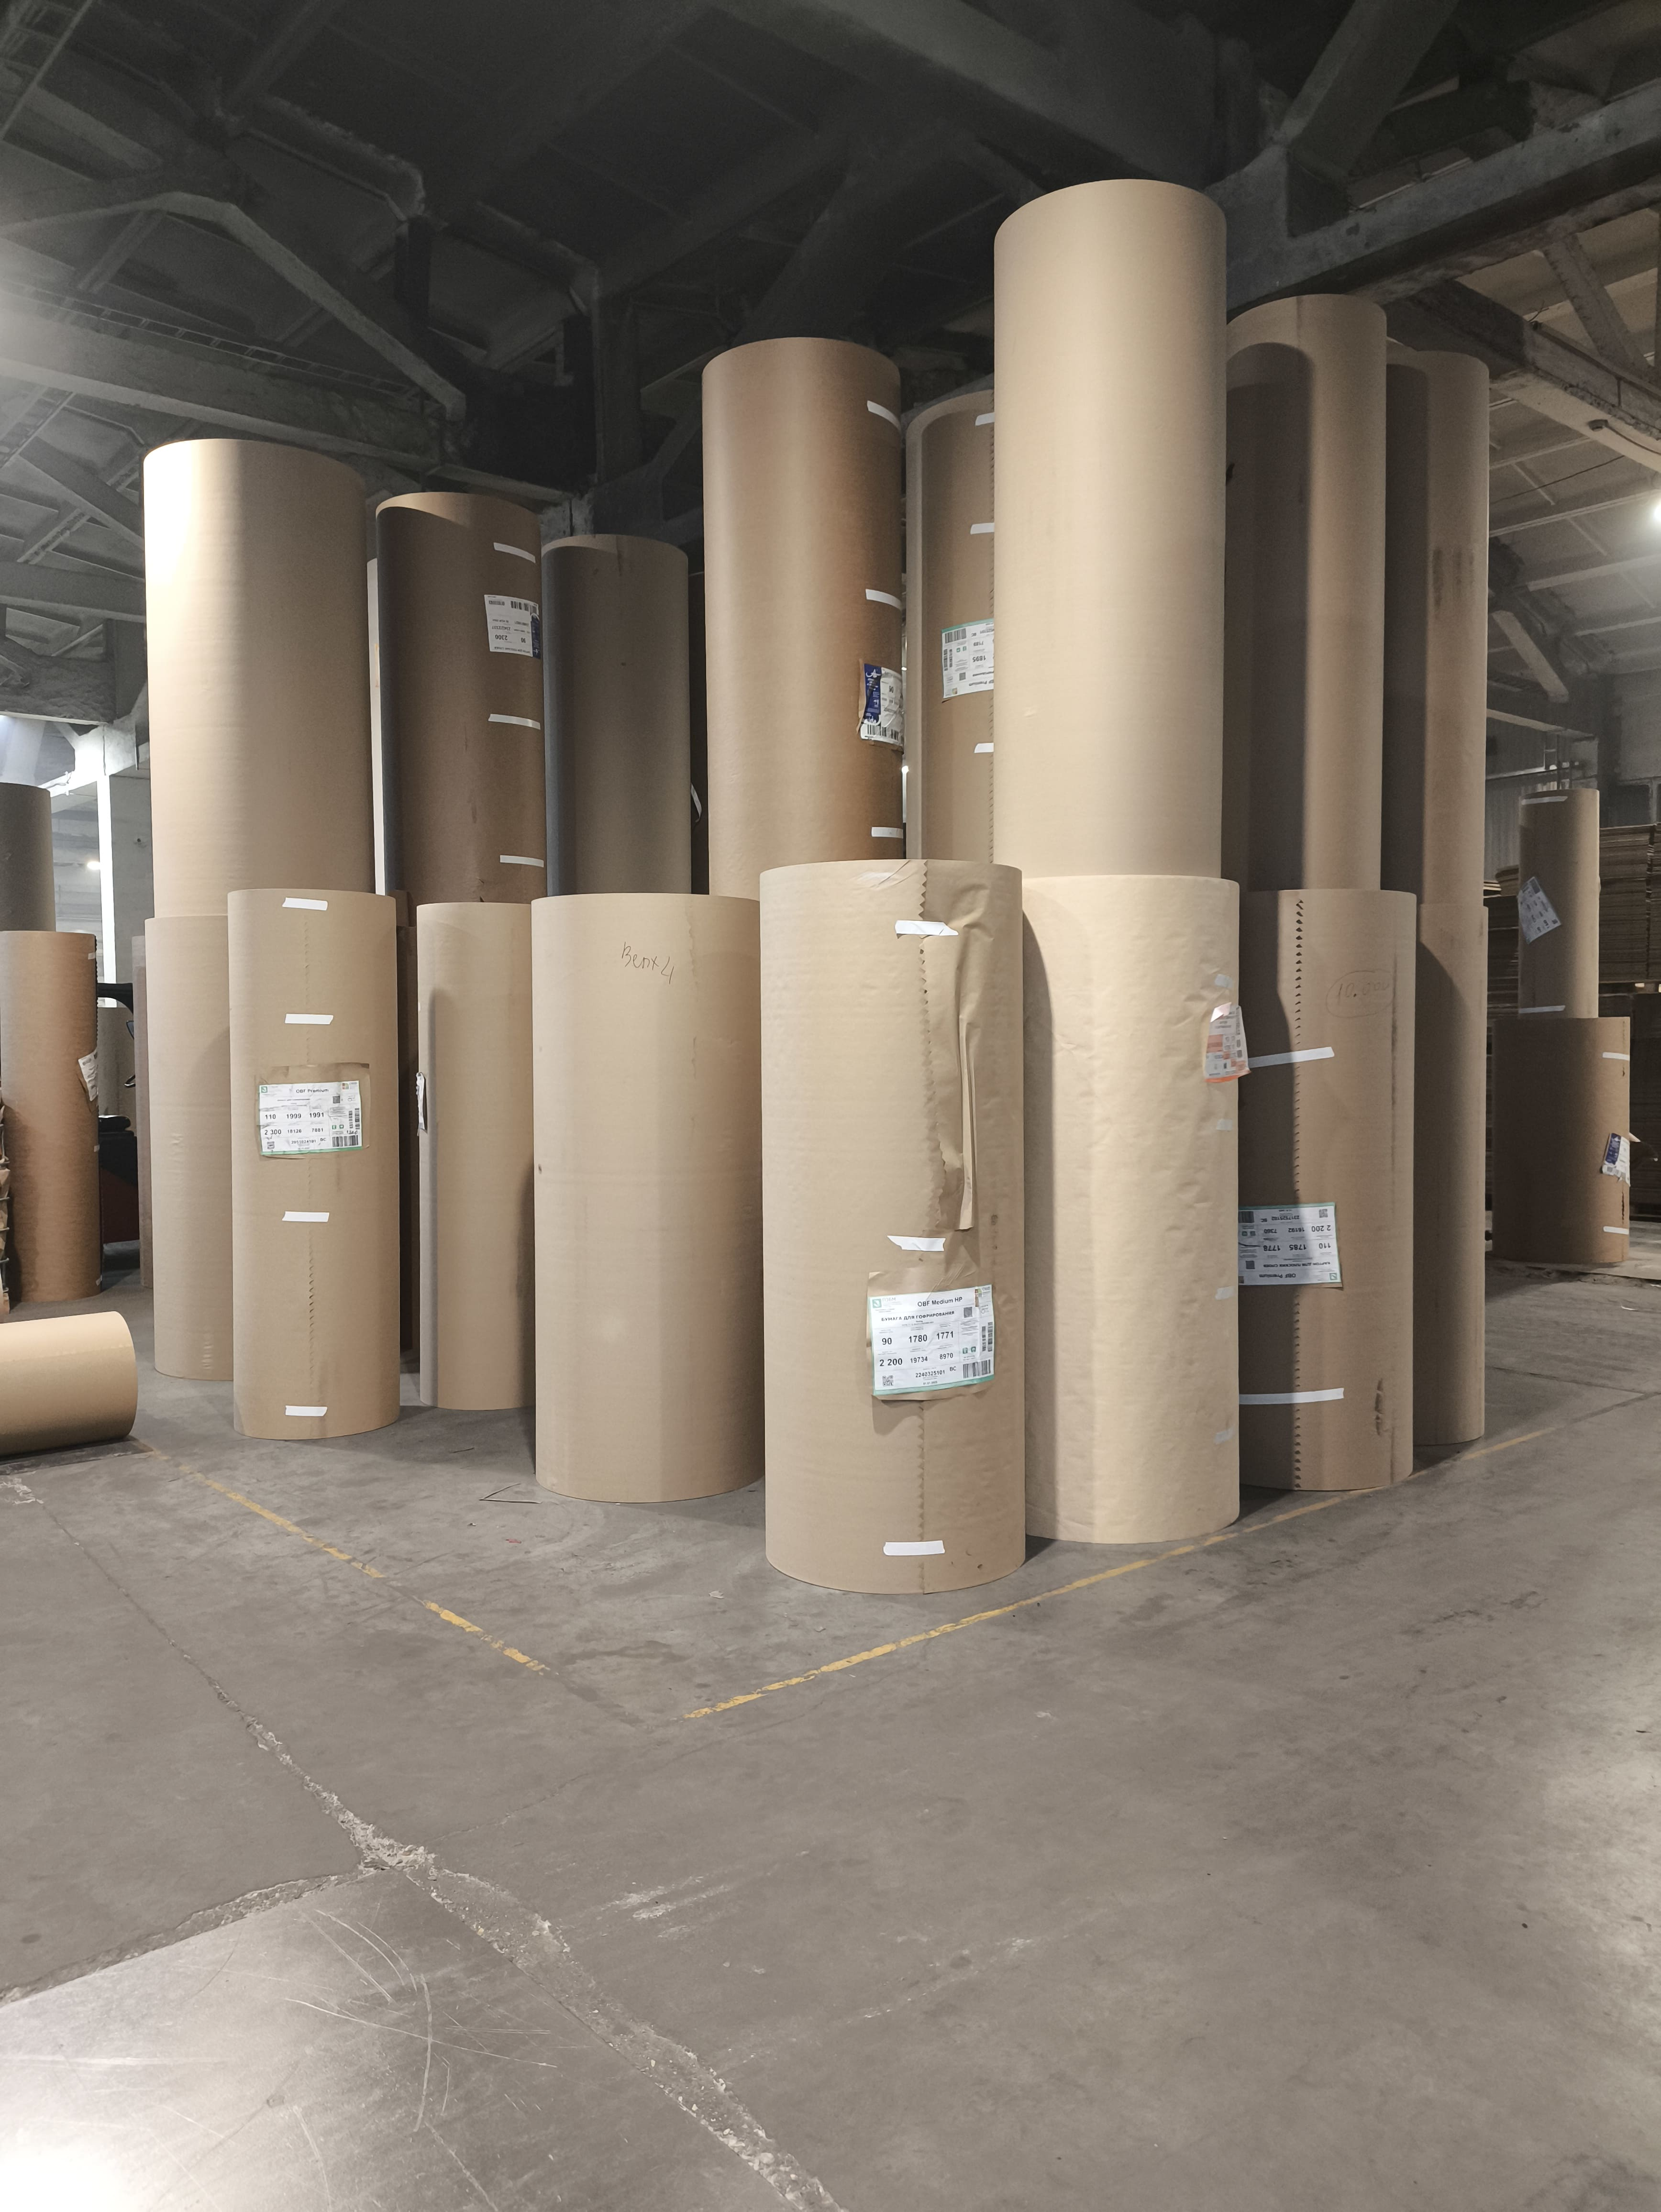
\includegraphics[height=0.4\textheight, keepaspectratio]{Pics/V недомоты.jpg}
\end{center}
 \caption{Хранение недомотов}
 \label{pic:V недомоты}
\end{figure}

\begin{figure}
\begin{center}
 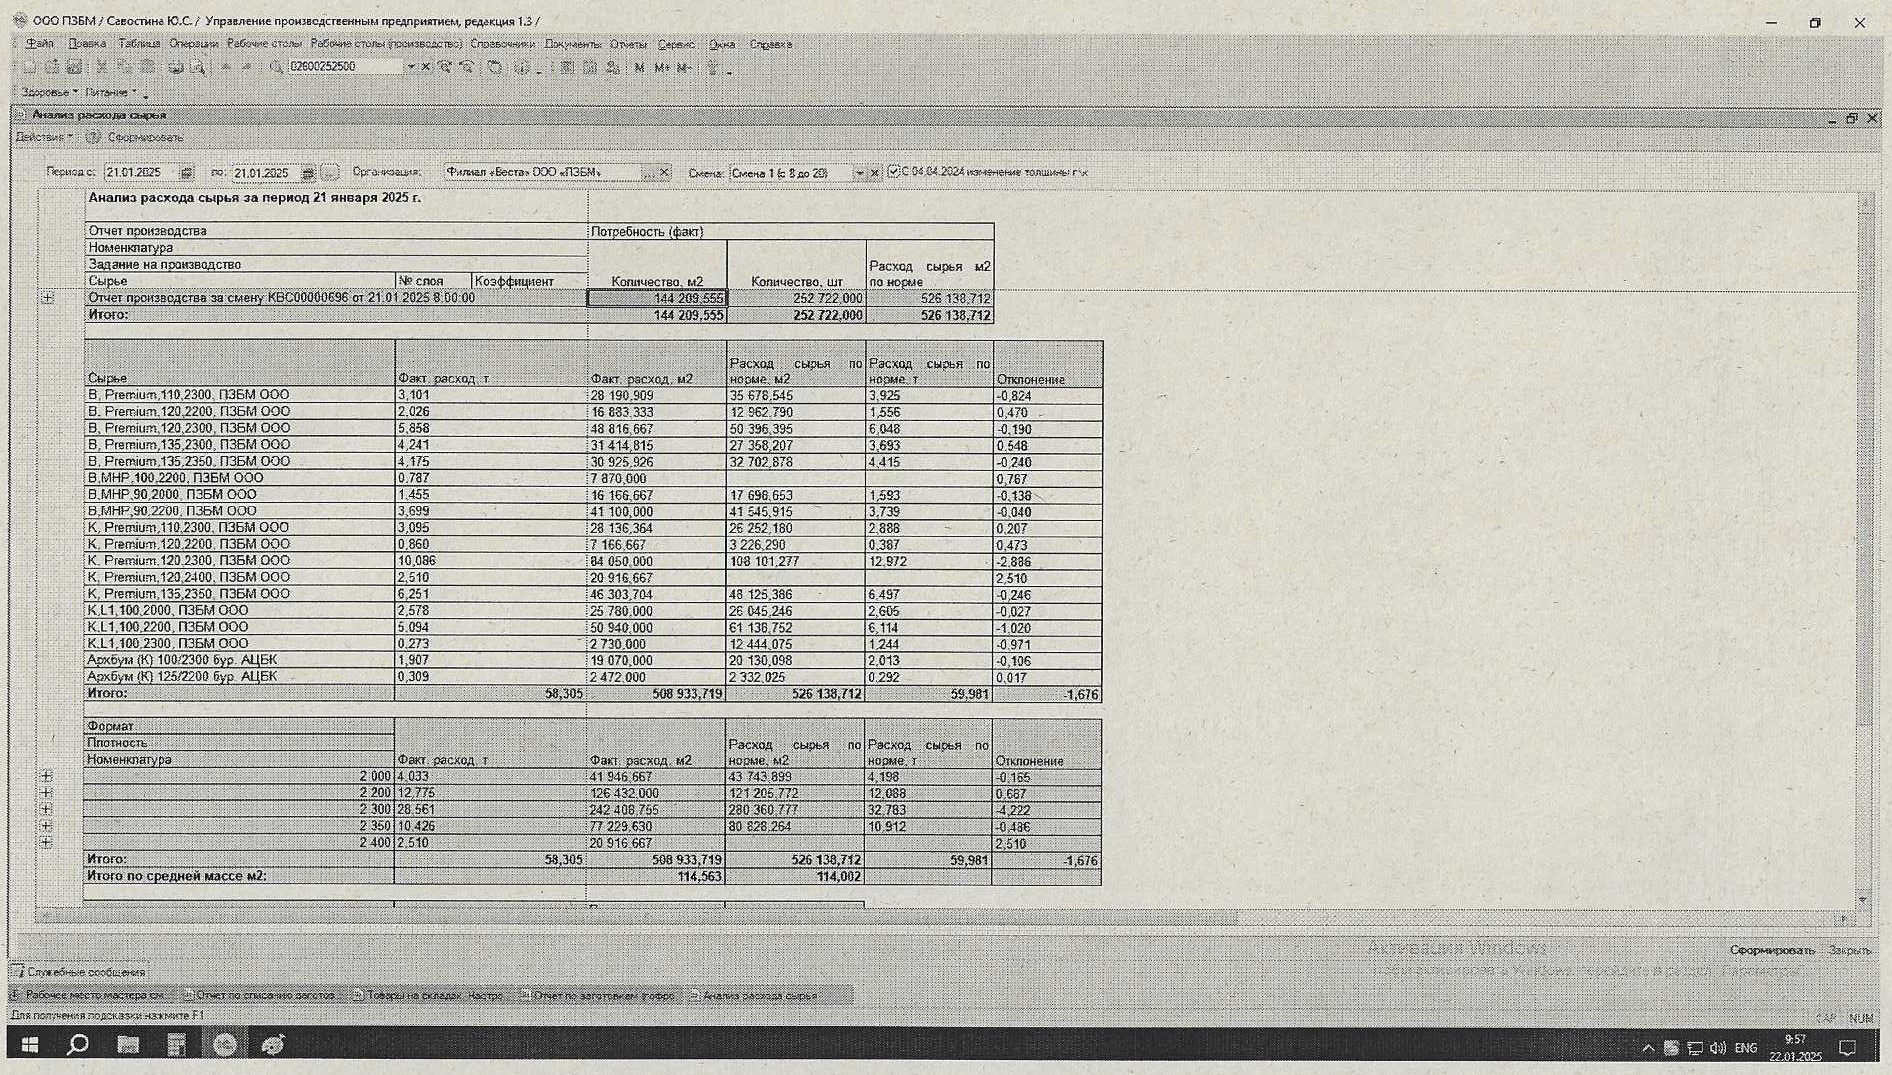
\includegraphics[height=0.37\textheight, keepaspectratio]{Pics/IV.2..jpg}
\end{center}
 \caption{Анализ расхода сырья}
 \label{pic:IV.2.}
\end{figure}

\begin{figure}
\begin{center}
 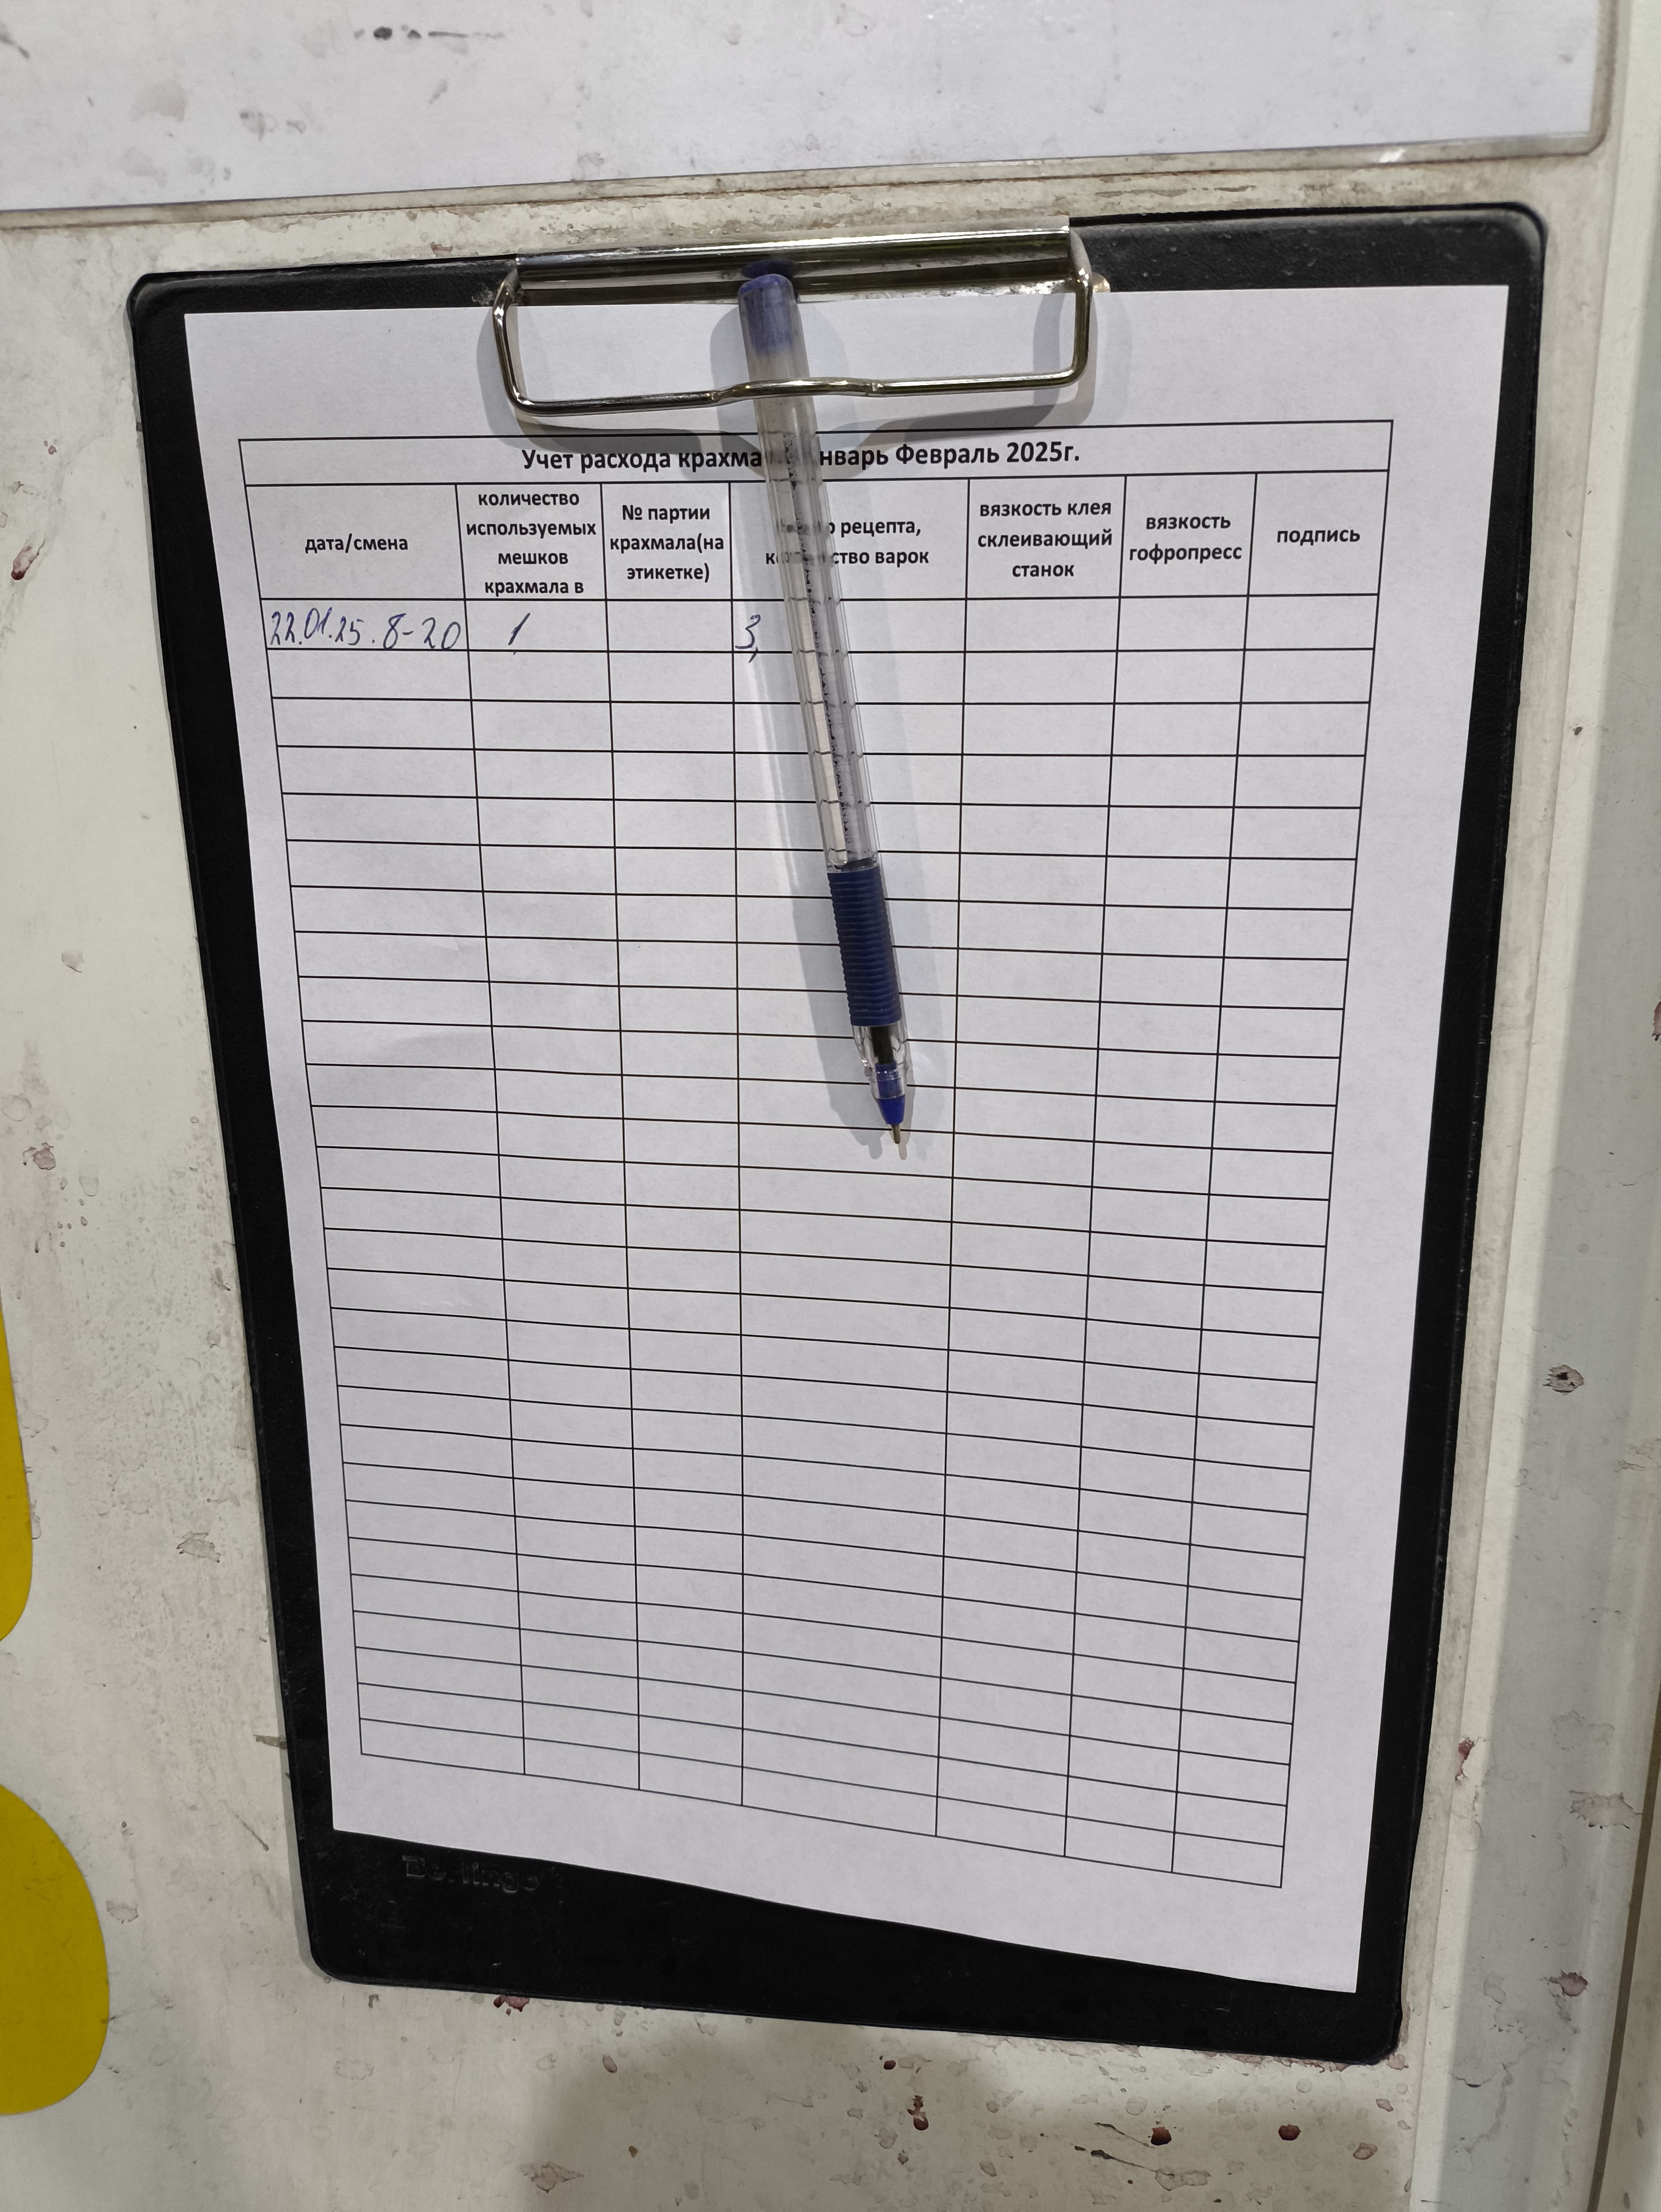
\includegraphics[height=0.9\textheight, keepaspectratio]{Pics/V учет расхода крахмала.jpg}
\end{center}
 \caption{Учет крахмала}
 \label{pic:V учет расхода крахмала}
\end{figure}
%\clearpage
%\ifx \notincludehead\undefined
\normalsize
\end{document}
\fi
\clearpage
\ifx \notincludehead\undefined
\normalsize
\end{document}
\fi

